\documentclass[12pt]{diploma}
%\pdfpkresolution=8000

\begin{document}

	\begin{titlepage}
		
\includepdf[pages=-,pagecommand={},scale=1]{title.pdf}
	\end{titlepage}
	
	\section*{Аннотация}
		
	В данной работе рассматривается вопрос программной реализации современных интеллектуальных алгоритмов кластер-анализа. Внимание уделено как теоретическому описанию эффективных алгоритмов, так и разработке программного кода модулей системы с дружелюбным графическим пользовательским интерфейсом. 
	
	Во введении обоснована необходимость создания разрабатываемого комплекса, описана текущая ситуация в области кластеризации и основные проблемы, возникающие при применении популярных алгоритмов кластеризации. 
	
	В теоретической части описаны пять реализованных алгоритмов: \ikmeans, \AWard, \AWardpb, \dePDDP, \BiKMR, указаны характерные свойства и математические приёмы, лежащие в основе каждого из них. Для прояснения наиболее сложных для понимания особенностей, некоторые алгоритмы разобраны на иллюстративных примерах. В конце теоретической части приводятся общие рекомендации по выбору наиболее подходящего алгоритма для различных случаев.
	
	В главе, посвящённой описанию программы вынесены вопросы взаимодействия с программой с точки зрения пользователя. Рассмотрены базовые операции и приведены пояснения к некоторым окнам графического интерфейса, с которыми сталкивается пользователь при выполнении этих операций. 
	
	Особенности программной реализации рассматриваются в главе \ref{sec:structure}. Эта глава содержит обоснование выбора средств реализации, и используемых программных библиотек. Некоторые вопросы освещены с помощью фрагментов кода. Для алгоритмов приведены схемы вычислений с необходимыми пояснениями.
	
	Для демонстрации принципов работы программы, особенностей предварительной подготовки данных и интерпретации результатов рассмотрен иллюстративный пример. На нем показаны полученные кластеры и изложена интерпретация каждого из кластеров в соответствии с характерными признаками.
	
	В заключении подведены итоги работы и обозначены возможные направления исследований и усовершенствований проекта.
	
	
		
	
	\tableofcontents 
	
	\newpage
		
	\section{Введение}
		В настоящее время наблюдается интенсивное развитие информационных технологий, появляются новые программные решения, применяемые в широком спектре областей. Если раньше информационные технологии были областью интересов узкого круга специалистов, то сейчас установилась тенденция к повсеместному распространению прикладных программных продуктов. 
		
		Современные компании вынуждены опираться на применение информационной инфраструктуры и использовать преимущества цифровых технологий для поддержания конкурентоспособности своих продуктов или услуг. В процессе эксплуатации информационных систем накапливаются массивы данных, обработка и интерпретация которых может принести компании коммерческую выгоду. 
		
		Каждый случай обработки данных, как правило, требует индивидуального подхода, не существует универсальной последовательности операций для любой задачи. Поэтому, обработка данных сопряжена с привлечением интеллектуальных усилий от высококвалифицированных специалистов. Программные системы анализа данных призваны облегчить этот труд и предоставляют в распоряжение специалиста наиболее востребованные процедуры обработки данных. Особенно актуально применение таких систем для решения прикладных задач, которые, несмотря на свою индивидуальность, зачастую однотипны и всё же имеют некоторые общие этапы решения. Применяя готовый, тщательно отлаженный и документированный программный код, сокращается время на анализ данных, а также снижается вероятность возникновения ошибок. 

		Прогресс технических средств в области сбора и обработки информации приводит к росту размеров массивов данных, которые требуется обрабатывать для удовлетворения потребностей компаний. Поэтому растёт роль методов агрегации данных и выделения в них общих закономерностей или структур. К таким методам, в частности относятся методы кластеризации. 
		
		Под кластеризацией понимают выделение объектов из таблицы наблюдений в множества, называемые кластерами, которые объединяют наиболее сходные объекты, при этом различные объекты должны попадать в разные кластеры \cite{mirkin-ds}. По принадлежности заданного нового объекта к определенному кластеру можно сделать предположения о его ключевых свойствах. Задачи кластеризации часто встают в самых разных областях, например, при обработке изображений или биологических структур а также социальных групп \cite{mirkin-clustering}.
		
		Вероятно, наиболее широко известный и популярный метод кластеризации --- \kmeans \cite{k-means-canonical}. Этот метод основан на поочерёдной минимизации квадратичного критерия по двум группам переменных: центрам кластеров и принадлежности объектов кластерам. На основе аналогичного квадратичного критерия предложены целый ряд эффективных алгоритмов, в том числе и иерархические, например, \Ward, \BisectingKmeans. 
		
		Однако, несмотря на популярность \kmeans, он обладает существенными недостатками. Первый заключается в том, что перед запуском алгоритма требуется знать число кластеров, которое должно быть выявлено. На практике, далеко не всегда число кластеров известно заранее. Например, в случае анализа интернет данных, сформированных из журналов посещений, и формирования групп схожих сайтов не предполагается наличие априорной информации. В таком случае придётся или рассматривать другие алгоритмы, или опираться на эмпирические зависимости.
		
		Второй недостаток заключается в том, что результат работы \kmeans сильно зависит от инициализации. В некоторых случаях неправильная инициализация может приводить к неудовлетворительным результатам. Этот недостаток обычно устраняют путём многократного запуска алгоритма для различных начальных условий, но при этом увеличивается и продолжительность кластеризации. Например, в случае обработки данных в режиме онлайн, такой способ может оказаться неприемлемым.  В то же время были предложены эффективные методы инициализации, которые позволяют оценить число кластеров с небольшими дополнительными временными затратами. 
		
		Третий существенный недостаток \kmeans состоит в снижении качества получаемого разбиения для случая зашумлённых данных. Многие данные, например составленные на основе измерений физических величин, содержат случайные погрешности, которые требуется учитывать при кластеризации для получения удовлетворительного результата. Отсутствие какого-либо механизма учёта шума в данных стимулирует исследователей предлагать усовершенствования \kmeans.
		
		Описанные выше недостатки \kmeans породили множество модификаций этого алгоритма, а также послужили импульсом для проведения работ над новыми алгоритмами, основанными на квадратичном критерии. Например, иерархический алгоритм \Ward \cite{ward-canonical} использует квадратичный критерий для агломеративного построения кластерной структуры. В совою очередь, \Ward также свойственны недостатки, которые частично были унаследованы от \kmeans, поэтому были предложены алгоритмы \Wardp и \AWardpb \cite{amorim-makarenkov-mirkin}, развивающие идею взвешенной кластеризации. Они продемонстрировали высокую эффективность при обработке зашумлённых данных, но, тем не менее, для канонической формулировки этих алгоритмов проблема выбора числа кластеров осталась неразрешенной. В дивизивных алгоритмах \BiKMR и \dePDDP \cite{kovaleva} используется автоматический критерий остановки, благодаря чему число кластеров определяется во время кластеризации.
		
		Таким образом, за последнее время появилось большое число новых и эффективных алгоритмов кластеризации, многие из них еще не реализованы в популярных библиотеках, таких как \texttt{scipy} для языка Python или  \texttt{Clustering Toolbox} для MATLAB. Авторы новых алгоритмов заявляют о их высокой эффективности и становится очевидно, что со временем эти алгоритмы найдут своё применение для задач определённой специфики. В данной работе рассматривается разработка программного обеспечения, в состав которого входит набор современных интеллектуальных алгоритмов кластеризации, основанных на критерии наименьших квадратов. Разработанная программа получила название ``Система интеллектуальной кластеризации данных'' (Intelligent Data Clustering Toolkit, INDACT).
		
		Программная система обладает графическим пользовательским интерфейсом, что делает её простой в применении даже для специалистов, не обладающих широкими познаниями в области программирования. В то же время пользовательский интерфейс представляет собой лишь надстройку над разработанной базовой библиотекой, которая включает в себя упомянутые алгоритмы. Эта библиотека имеет открытый код, снабжённый необходимой документацией, и тем самым допускает использование в других программных продуктах. 
		
	\section{Теоретическая часть}
	
	В теоретической части будут подробно описаны основные алгоритмы, реализованные в системе INDACT. Алгоритмы кластеризации по принципу работы разделяют на две категории: плоские и иерархические. К плоским относится, например, популярный \kmeans. Данная работа затрагивает в основном вторую категорию. Иерархические алгоритмы, в отличие от плоских, формируют вложенную структуру кластеров. Информация о взаимной вложенности кластеров может быть полезна для некоторых практических приложений, например, при исследовании биологических видов, вложенность кластеров может отражать филогенетическое родство. Это интересное свойство повышает интерес исследователей к иерархическим алгоритмам.
	
	Различают два вида иерархических алгоритмов: агломеративные (объединяющие) и дивизивные (разделяющие), которые соответственно реализуют восходящее и нисходящее направление формирования результирующего разбиения. Агломеративные алгоритмы рассматривают исходные данные как множество кластеров, состоящих из единственного объекта, который одновременно является центром. Итеративно происходит объединение двух ближайших кластеров, пока не будет выполнен заданный критерий останова. Дивизивные алгоритмы в противоположность агломеративным начинают работу с одного кластера, в который включены все объекты данных и разделяют его на более мелкие кластеры. 
	
	Программная система INDACT предоставляет пользователю выбор из четырёх современных алгоритмов кластеризации, два из которых агломеративные, а два --- дивизивные. Агломеративные алгоритмы \AWard и \AWardpb основаны на классическом критерии Ward, но расширяют традиционный подход с помощью предварительного этапа, называемого аномальной кластеризацией. Задача аномальной кластеризации состоит в предварительной разведке кластерной структуры и вычленении аномальных кластеров, которые расположены далеко от центра данных. Алгоритм \AWardpb, кроме того, предполагает взвешивание признаков, что может рассматриваться как механизм учёта случайных погрешностей. Два дивизивных алгоритма --- \dePDDP и \BiKMR используют автоматические критерии останова, выполнение которых проверяется на каждой итерации. Они хорошо подходят для тех случаев, когда число кластеров заранее неизвестно.
	
	Кроме кластеризации в состав программной системы включён модуль для генерации данных. Этот модуль позволяет сгенерировать при помощи небольшого числа управляющих параметров синтетические данные и на их примере проверить работу различных алгоритмов.

	\subsection{Постановка задачи кластеризации}
	В  работе используется представление данных в виде таблицы объект--признак. Такой формат данных широко распространён для практических приложений и встречается во многих реальных ситуациях. Программа INDACT не позволяет обрабатывать другие варианты представления данных. 
	
	Пусть имеется $ N $ объектов и у каждого объекта определены значения $ V $ признаков. Вообще говоря, признаки могут принимать как числовые значения, так и номинальные. Далее подразумевается, что если исходные данные имеют номинальные признаки, то их следует представить с помощью выбранного метода в виде числовых значений. Например, номинальный признак может быть разложен на несколько бинарных, каждый бинарный признак обозначает наличие (значение 1) или отсутствие (значение 0) соответствующего значения исходного признака.
	Множество всех объектов будем обозначать $ Y $. Тогда эти данные могут быть представлены в виде таблицы следующего вида:
	
	\begin{equation*}
	Y= \begin{pmatrix} 
	y_{1} \\
	\cdots \\ 
	y_{N} 
	\end{pmatrix}
	= \begin{pmatrix} 
	y_{11} & \cdots  & y_{1V} \\ 
	\cdots & \cdots  & \cdots \\ 
	y_{N1} & \cdots  & y_{NV} 
	\end{pmatrix}
	\end{equation*}
	
	Требуется получить разбиение $ S = \{C_1,\ldots,C_K\} $, состоящее из $ K $ кластеров, которые не пересекаются и покрывают всё множество объектов $ Y $. Кластер будем обозначать прописной буквой $ C $, а его центр --- строчной $ c $. В общем случае значение $ K $ не известно, хотя встречаются ситуации в которых число кластеров задано. Например, число кластеров может быть известно исходя из общих закономерностей предметной области. Чёткой формулировки относительно того, что должно быть включено в кластеры не существует. Общая идея состоит в том чтобы сходные объекты были включены в один кластер, а несходные не принадлежали одному кластеру. В схожесть объектов в различных приложениях может вкладываться различный математический смысл, например, схожесть объектов может определяться геометрической близостью или совпадением некоторых основных переменных.

	\subsection{Аномальная кластеризация} \label{subsec:anomalous}
	Аномальная кластеризация \cite{anomalous-clustring} имеет большое значение для всего программного комплекса, так как этот подход широко используется как составляющая часть более сложных алгоритмов, например, аномальная инициализация является первым шагом \AWard и \AWardpb. Этот этап позволяет предварительно ``разведать'' структуру данных и тем самым сформировать исходные предположения о возможном числе кластеров. 
	
	Алгоритмы, основанные на \kmeans требуют явного задания числа кластеров и начальных центров. Как правило, число кластеров определяется исходя из общих зависимостей и представлений пользователя о предметной области. Начальные центры кластеров определяются по результатам нескольких запусков для случайного положения с последующим выбором наилучшего результата. Зачастую у пользователя не имеется никаких представлений о предметной области относительно возможного числа кластеров. Поэтому в настоящее время идёт интенсивная работа над разработкой различных методов, которые позволяли бы определить число кластеров исходя исключительно из самих данных. 
	
	Аномальный кластер-анализ является одним из таких методов. Он основан на поочерёдном поиске аномальных групп и исключении их из данных, до тех пор, пока не останется ни одного объекта. Под аномальной группой понимается множество объектов, которые далеко отстоят от глобального центра данных.  Количество найденных аномальных групп объектов может служить приближением числа кластеров. Существуют алгоритмы, которые непосредственно используют найденное число кластеров в результате аномальной инициализации, например, \ikmeans \cite{anomalous-clustring}, а также алгоритмы, которые только опираются на этот результат для первой итерации и могут производить отличное число кластеров, например, \AWardpb.
	
	Метод аномальных кластеров можно рассматривать как модифицированный частный случай \kmeans при числе кластеров $ K=2 $. При этом инициализация начального положения центров кластеров жёстко определена --- один кластер всегда имеет центр в глобальном центре всех данных и не изменяется во время работы алгоритма, а центр второго кластера, который называется аномальным, инициализируется в наиболее удалённой от глобального центра точке. В процессе работы центр аномального кластера уточняется аналогично традиционному \kmeans. Отличие метода аномальных кластеров от \kmeans заключается в том, что один центр остаётся неизменным при на всех итерациях. На каждом шаге в аномальный кластер включаются те точки, которые лежат ближе к центру аномального кластера, чем к глобальному центру данных. После центр аномального кластера обновляется чтобы соответствовать среднему по всем включённым объектам. Когда центр аномального кластера стабилизировался и не изменяется, происходит исключение найденного кластера и продолжается работа с оставшимися данными. Исключение аномальных групп объектов происходит до тех пор, пока не останется ни одного объекта. 
	
	Формально алгоритм аномального кластер-анализа можно записать в следующем виде:
	
	\begin{algorithm}{Аномальная кластеризация (ik-means)}{ikmeans}	
%		\label{alg:ikmeans}
		\begin{astep}{Подготовка}
			Задаться пороговым значением минимальной численности аномального кластера $ \Theta $. Вычислить глобальный центр данных $ a = (a_1,\ldots,a_V) $:
			\begin{equation*}
				a_v=\frac{1}{N} \sum_{i=1}^{N}y_{iv}
			\end{equation*}
			Если имеются исходные представления о норме, использовать их для вычисления глобального центра. Стандартизировать таблицу данных сдвигом начала координат в точку $ a $.
		\end{astep}
		\begin{astep}{Инициализация аномального центра \label{itm:alg-anomal-init-center}}
			Определить наиболее удалённую от начала координат точку $ c $. Эта точка является начальным центром аномального кластера. 
		\end{astep}
		\begin{astep}{Обновление аномального кластера \label{itm:alg-anomal-update-cluster}}
			Объекты, которые расположены ближе к центру $ c $, чем к началу координат включить в аномальный кластер. Если в аномальный кластер не было внесено изменений, перейти к шагу  \ref{itm:alg-anomal-save-centroid}.
		\end{astep}
		\begin{astep}{Обновление центра \label{itm:alg-anomal-update-center}}
			Вычислить новый центр аномального кластера как покомпонентное среднее всех объектов, включённых в него.  Перейти к шагу \ref{itm:alg-anomal-update-cluster}.
		\end{astep}
		\begin{astep}{Сохранение центра \label{itm:alg-anomal-save-centroid}}
			Если число объектов в аномальном кластере больше заданного порогового значения $ \Theta $, сохранить центр и ассоциированный с ним аномальный кластер в список результатов.
		\end{astep}
		\begin{astep}{Исключение аномального кластера}
			Исключить из данных все объекты, которые принадлежат аномальному кластеру.  Если в таблице $ Y $ все ещё остаются объекты, прейти к шагу \ref{itm:alg-anomal-init-center}.
		\end{astep}
		\begin{astep}{Кластеризация}
			Выполнить алгоритм \kmeans \cite{k-means-canonical} на исходных данных $ Y $. При этом использовать центры аномальных кластеров, сохранённых на шаге \ref{itm:alg-anomal-save-centroid} в качестве начальных. Результатом работы \ikmeans является полученное разбиение.
		\end{astep}
	\end{algorithm}

	В \cite{mirkin-ds} показано, что аномальная кластеризация минимизирует критерий, подобный критерию метода \kmeans:
	\begin{equation*}
		W(S,c) = \sum_{i \in C}^{} d(y_i,c) + \sum_{i \notin C}^{} d(y_i,0),
	\end{equation*}
	\begin{conditions}
		 C     &  искомый кластер; \\
		 c     &  центр кластера $ С $; \\
		 d     &  квадрат евклидовского расстояния.\\  
	\end{conditions}

	\begin{figure} % \ContinuedFloat
		\centering
		\subfigure[Исходные данные] {\label{fig:ikmeans1}\includestandalone[width=0.49\textwidth]{tikz/v2/ik-means/ik-means-1}}
		\subfigure[Выбор начального центра аном. кластера] {\label{fig:ikmeans2}\includestandalone[width=0.49\textwidth]{tikz/v2/ik-means/ik-means-2}}
		\subfigure[Аномальный кластер сформирован] {\label{fig:ikmeans3}\includestandalone[width=0.49\textwidth]{tikz/v2/ik-means/ik-means-4}}
		\subfigure[Аномальный кластер исключён] {\label{fig:ikmeans4}\includestandalone[width=0.49\textwidth]{tikz/v2/ik-means/ik-means-5}}
		\subfigure[Итоговое разбиение аном. кластерами] {\label{fig:ikmeans5}\includestandalone[width=0.49\textwidth]{tikz/v2/ik-means/ik-means-22}}
		\subfigure[Результат после выполнения \kmeans] {\label{fig:ikmeans6}\includestandalone[width=0.49\textwidth]{tikz/v2/ik-means/ik-means-23}}
		\caption{\ikmeans: этапы выделения аномальных кластеров
			\\ {\small Каждому кластеру соответствуют точки определённого цвета в двумерном пространстве.}}
		\label{fig:ikmeans-working}
	\end{figure}

	Стоит заметить, что хотя аномальная кластеризация и позволяет предварительно ``разведать'' структуру данных, но на применение этого метода также имеются ограничения. Например, следует учитывать, что получаемая структура аномальных кластеров сгущается ближе к началу координат. Для сглаживания этого недостатка рекомендуется отбрасывать слишком маленькие аномальные группы, число объектов в которых меньше заданного значения $ \Theta $. 
	
	Рассмотрим работу алгоритма \ikmeans на простом примере. Пусть имеются двумерные данные, изображённые на рисунке \ref{fig:ikmeans1}. Первым шагом алгоритм определяет наиболее удалённую точку от глобального центра данных (на рисунке \ref{fig:ikmeans-working} обозначается чёрной звёздочкой) как показано на рисунке \ref{fig:ikmeans2}. Когда начальный центр аномального кластера определён, выполняются шаги некоторой вариации \kmeans при $ K=2 $ и жёстко зафиксированным центром данных. При этом центр аномального кластера уточняется до схождения (рисунок \ref{fig:ikmeans3}). Объекты, которые находятся ближе к центру аномального кластера, чем к глобальному центру исходных данных, включаются в состав аномального кластера и на после схождения очередной итерации, исключаются из данных без изменения глобального центра (см. рисунок \ref{fig:ikmeans4}). Когда все объекты будут исчерпаны, для полученных аномальных кластеров выполняется классическая версия \kmeans с числом кластеров, равным числу найденных аномальных групп и соответствующими центрами. Результат работы \ikmeans изображён на рисунке \ref{fig:ikmeans6}.	
	
	Метод аномальной кластеризации позволяет достичь хороших результатов, но как было показано в недавних исследованиях \cite{amorim-makarenkov-mirkin}, в случае задания стандартного порогового параметра $ \Theta=1 $, выделяет избыточное число кластеров. Определение рационального значения $ \Theta $ в настоящее время не имеет методической поддержки, поэтому для использования большого потенциала алгоритма было предложено его новое применение в роли предварительного этапа инициализации иерархических алгоритмов. 
		
	
	\subsection{Алгоритм \AWard}
	Алгоритм \AWard является модернизацией широко известного алгоритма иерархической кластеризации \Ward. Алгоритм \Ward \cite{ward-canonical} относится к агломеративным, то есть он действует по принципу ``снизу вверх''. На первом этапе принимается, что каждый отдельный объект $ y_i \in Y $ представляет собой кластер, центром которого является сам объект $ y_i $. Алгоритм \Ward итеративно выбирает два ближайших кластера и объединяет их, таким образом уменьшая общее число кластеров на единицу на каждой итерации. Процесс повторяется, пока не будет достигнуто заранее заданное число кластеров. Опишем последовательность шагов \Ward:
	\begin{algorithm}{Ward}{}	
		\begin{astep}{Инициализация}
			Задаться желаемым числом кластеров $ K^* $. Установить начальное число кластеров равным числу объектов $ K=N $. Исходное разбиение образованно элементарными кластерами $ S=\{C_1,\ldots,C_K\} $, в каждый из которых включён единственный объект $ y_i \in Y $ из исходных данных.
		\end{astep}
		\begin{astep}{Слияние кластеров \label{itm:ward-merge}}
			Выбрать два ближайших кластера $ C_a, C_b \in S $ согласно следующей формуле:
			\begin{equation}\label{eq:ward-dist}
				d_{Ward}(C_a,C_b) = \frac{N_1 N_2}{N_1 + N_2} \sum_{v=1}^{V} (c_{av}-c_{bv})^2,
			\end{equation}
			\begin{conditions}
				N_1,N_2       &  число объектов в кластерах $ C_a, C_b $; \\
				c_{av},c_{bv} &  $ v $-ая координата центра кластеров  $ C_a, C_b $. \\
			\end{conditions}
			
			Сформировать новый кластер $ C_{ab} $, в который входят все объекты из $ C_a $ и $ C_b $, удалив при этом старые кластеры $ C_a, C_b $.	Уменьшить текущее число кластеров $ K $ на 1. 
		\end{astep}
		\begin{astep}{Обновление центра}
			Вычислить новый центр сформированного кластера $ C_{ab} $ как покомпонентное среднее среди всех объектов этого кластера.
		\end{astep}
		\begin{astep}{Условие остановки}
			Если текущее число кластеров больше желаемого $ K>K^* $ и $ K>1 $, перейти к шагу \ref{itm:ward-merge}. В противном случае выдать текущее разбиение в качестве результата.
		\end{astep}
	\end{algorithm}

	Следует обратить внимание на два важных свойства алгоритма \Ward. Во-первых, как и любой иерархический алгоритм, \Ward формирует вложенную структуру классов, что может быть использовано в некоторых практических приложениях, где вложенность кластеров может быть естественным образом объяснена в терминах предметной области. Во-вторых, в канонической формулировке алгоритм не требует инициализации, как например, \kmeans. Таким образом, отпадает необходимость многократного запуска для определения наилучшего разбиения при различных начальных условиях.
	
	Но у \Ward есть существенный недостаток --- это продолжительность вычислений. В соответствии с описанной последовательностью шагов на каждой итерации алгоритма происходит вычисление расстояния между всеми кластерами. На первых итерациях число кластеров примерно равно числу объектов, это значит что требуется время, квадратично зависящее от $ N $. Этот недостаток послужил толчком для исследования возможности применения аномальной кластеризации для сокращения вычислений. 
	
	Из экспериментальных исследований известно, что аномальная кластеризация порождает избыточное число кластеров в то время как \Ward на каждом шаге сокращает число кластеров на единицу. Сочетание аномальной кластеризации и алгоритма \Ward позволит сократить время вычисления благодаря исключению стадии с большим числом маленьких кластеров. Такая модификация получила название \AWard \cite{amorim-makarenkov-mirkin}. 
	\begin{algorithm}{A-Ward}{}
		\begin{astep}{Инициализация \label{itm:a-ward-init}}
			Установить $ \Theta=1 $. Получить начальное число кластеров $ K $ и само разбиение  $ S $ по алгоритму \ikmeans (алгоритм  \ref{alg:ikmeans}).
		\end{astep}		
		\begin{astep}{Слияние кластеров \label{itm:a-ward-merge}}
			Выбрать два ближайших кластера $ C_a, C_b \in S $ согласно формуле \eqref{eq:ward-dist}.			
			Сформировать новый кластер $ C_{ab} $, в который входят все объекты из $ C_a $ и $ C_b $, удалив при этом старые кластеры $ C_a, C_b $.	Уменьшить текущее число кластеров $ K $ на 1. 
		\end{astep}
		\begin{astep}{Обновление центра}
			Вычислить новый центр сформированного кластера $ C_{ab} $ как покомпонентное среднее среди всех объектов этого кластера.
		\end{astep}
		\begin{astep}{Условие остановки}
			Если текущее число кластеров больше желаемого $ K>K^* $ и $ K>1 $, перейти к шагу \ref{itm:a-ward-merge}. В противном случае выдать текущее разбиение в качестве результата.
		\end{astep}
	\end{algorithm}
	
	На рисунке \ref{fig:ward-working} продемонстрирован принцип работы алгоритма \AWard для простых двумерных данных. Пусть после выполнения шага \ref{itm:a-ward-init} была получена кластерная структура, показанная на рисунке \ref{fig:ward1}. Исключительно в целях демонстрации зададим $ K^*=1 $, то есть алгоритм продолжит работать пока не будет сформирован единственных кластер из всех объектов. Предположим что, после сравнения всех расстояний между кластерами, вычисленных по формуле \eqref{eq:ward-dist} выяснилось, что красный и синий кластеры имеют наименьшее расстояние. Тогда они будут объединены в один кластер (для определённости присвоим ему красный цвет, хотя это не имеет значения). На следующем этапе будет произведено сравнение расстояний между оставшимися четырьмя кластерами и объединение ближайших, как показано на рисунке \ref{fig:ward2}. Объединение кластеров продолжится, пока два последних кластера не будут слиты в единый \ref{fig:ward5}. Схематично процесс слияния кластеров можно изобразить дендограммой \ref{fig:ward6}, которая показывает на каком этапе какие кластеры были объединены. Процесс иерархического кластер-анализа удобен с точки зрения остановки процесса: её можно произвести на любом этапе по заданному критерию, получив при этом соответствующее число кластеров. Таким образом, если было бы определено желаемое число кластеров, например, равное трём, процесс был бы остановлен через две итерации и результирующему разбиению соответствовала бы картинка \ref{fig:ward3}.
	
	Предложенное усовершенствование позволяет существенно сократить время работы алгоритма, благодаря исключению трудоёмких начальных стадий с большим числом кластеров. Вместо исходного элементарного разбиения используется предварительно найденные аномальные кластеры, число которые существенно меньше числа объектов.

	\begin{figure} % \ContinuedFloat
		\centering
		\subfigure[Первое объединение (синее и красное)] {\label{fig:ward1}\includestandalone[width=0.49\textwidth]{tikz/ward/ward1}}
		\subfigure[Второе объединение (зелёное и бирюзовое)] {\label{fig:ward2}\includestandalone[width=0.49\textwidth]{tikz/ward/ward2}}
		\subfigure[Третье объединение (зелёное и коричневое)] {\label{fig:ward3}\includestandalone[width=0.49\textwidth]{tikz/ward/ward3}}
		\subfigure[Четверное объединение (зеленое и красное)] {\label{fig:ward4}\includestandalone[width=0.49\textwidth]{tikz/ward/ward4}}
%		\subfigure[Процесс остановлен] {\label{fig:ward5}\includestandalone[width=0.49\textwidth]{tikz/ward/ward5}}
		\subfigure[Дерево вложенности кластеров] {\label{fig:ward6}\includestandalone[width=0.49\textwidth]{tikz/ward/ward-tree}}
		\caption{\AWard: этапы объединения кластеров, полученных в результате применения \ikmeans
			\\ {\small Каждому кластеру соответствуют точки определённого цвета в двумерном пространстве. Объединение кластеров обозначено серым затемнением с пунктирными границами.  На дендограмме цвет ветви соответствует цвету точек кластера.}}
		\label{fig:ward-working}
	\end{figure}
	
	\subsubsection{Специальный критерий остановки}
	В той формулировке алгоритма \AWard, которая была приведена выше не удаётся избавиться от традиционного недостатка, присущего многим алгоритмам, основанных на \kmeans. Этот недостаток заключается в необходимости задать желаемое число кластеров. Однако, в направлении разрешения этой проблемы был сделан вклад в работе \cite{spec-criterion}, в которой предложен специальный критерий остановки алгоритма. Предлагаемый способ завершения кластеризации в общем случае применим для иерархических алгоритмов с квадратичным критерием минимизации:
	\begin{equation} \label{eq:square-criterion}
		W(S,c) = \sum_{k=1}^{K} \sum_{i \in C_k}^{} \sum_{v=1}^{V} (y_{iv} - c_{kv})^2,
	\end{equation}
	\begin{conditions}
		W       & минимизируемый квадратичный критерий; \\
		S       & кластерное разбиение, $ S={C_1,\ldots,C_K} $; \\	
		K       & число кластеров, $ K = |S| $; \\
		C_k     & $ k $-ый кластер разбиения; \\
		c_{kv}  & $ v $-ая координата центра $ k $-го кластера; \\
		y_{iv}  & $ v $-ая координата центра $ i $-го объекта; \\
	\end{conditions}
	
	Пусть на некотором этапе работы происходит объединение некоторых двух кластеров $ C_k $ и $ C_l $ с формированием нового кластера $ C_{kl} $. Его центр можно вычислить по формуле: $ c_{kl} = (N_k \cdot c_k + N_l \cdot c_l)/(N_k + N_l) $, где $ N_k $ и $ N_l $ обозначают число объектов в кластерах $ C_k $ и $ C_l $ соответственно. При объединении кластеров происходит увеличение критерия \eqref{eq:square-criterion} на величину $ \Delta $:
	\begin{equation} \label{eq:spec-criterion-delta}
		\Delta(k,l) = W(S(k,l),c(k,l)) - W(S,c),
	\end{equation}
	\begin{conditions}
		S(k,l)       & разбиение, полученное из $ S $ разбиения после слияния кластеров $ C_k $ и $ C_l $; \\
		c(k,l)       & центры кластеров соответствующих разбиению $ S(k,l) $; \\
	\end{conditions}
	Величина $ \Delta $ всегда положительна, поскольку квадратичный критерий \eqref{eq:square-criterion} уменьшается с ростом числа кластеров и достигает нуля при $ K = N $. Величину изменения квадратичного критерия можно выразить через характеристики объединяемых кластеров:
	\begin{equation*}
		\Delta(k,l) = \frac{N_k N_l}{N_k + N_l}d(c_k,c_l)		
	\end{equation*}
	
	Как было отмечено в упомянутой статье \cite{spec-criterion}, при вычислении приращения квадратичного критерия \eqref{eq:square-criterion}  по формуле \eqref{eq:spec-criterion-delta} взаимно обнуляются все слагаемые, за исключением тех, которые относятся к кластерам $ C_k $, $ C_l $, $ C_{kl} =C_k \cup C_l $. Таким образом, можно переписать выражение \eqref{eq:spec-criterion-delta} следующим образом: $ 		\Delta(k,l) = w(C_k \cup C_l) - w(C_k) - w(C_l) $, где $  w(C) = \sum_{i\in C}^{} d(y_i,c) $ --- сумма квадратов евклидовских расстояний от точек кластера до его центра. 
	
	Предлагаемый специальный критерий имеет вид:
 	\begin{equation*}
	 	\Delta(k,l) < \alpha\:w(C_k \cup C_l)
 	\end{equation*}
 	где $ \alpha=\dfrac{1}{2} $.
	
	\subsection{Алгоритм \AWardpb}
		В реальный приложениях требуется анализировать данные с зашумлёнными признаками, которые были получены путём измерения некоторых физических параметров. В этом случае у алгоритмов \Ward и \AWard появляется неспособность отделения существенных признаков от шумовых. Для снижения влияния нерелевантных признаков предлагается ввести весовые коэффициенты, которые вычисляются на основании разброса значений признака: чем разброс больше, тем меньшую роль играет этот признак при кластеризации. 
		
		Модификация алгоритма \AWard, учитывающая вес признака получила название \AWardpb. В этой модификации также учтено обобщение для использования метрики Минковского произвольной степени. В обозначении алгоритма указано два параметра, буква $ p $ указывает на возможность изменения степени Минковского, а $ \beta $ --- степени весовых коэффициентов.
		
		Как и в случае с \AWard, для ускорения работы используется аномальная кластеризация. Алгоритм \AWardpb потребовал разработки обобщённой версии метода аномального кластер-анализа с использованием весовых коэффициентов и для заданной метрики Минковского. Ниже описана версия алгоритма \ref{alg:ikmeans} для использования с алгоритмом \AWardpb:
		
		\begin{algorithm}{Аномальная инициализация для $ A-Ward_{p\beta} $}{awardpb-init}
			\begin{astep}{Инициализация}
				Задаться значениями параметров $ p $ и $ \beta $. Вычислить глобальный центр данных $ c_Y $ как покомпонентный центр Минковского по всем объектам $ y_i \in Y $.
			\end{astep}
			\begin{astep}{Определение центра аномального кластера} \label{itm:awardpb-init-center}
				Аномальный кластер принять пустым, $ C_t = \varnothing $. Весовые коэффициенты распределить равномерно по всем признакам $ w_{kv} = 1/V $ при $ k=1,2 $ и $ v=1,\ldots,V $. За центр аномального кластера принять объект, который наиболее удалён от глобального центра $ c_Y $ по взвешенной метрике Минковского:
				\begin{equation} \label{eq:weighted-mink}
					d_{p\beta}(y_i, c_k) = \sum_{v=1}^{V}w^\beta_{kv}|y_{iv}-c_{kv}|^p
				\end{equation}
			\end{astep}
			\begin{astep}{Обновление аномального кластера}
				Каждый объект, который находится ближе к центру аномального кластера $ c_t $, чем к глобальному центру данных $ c_Y $, приписать к кластеру $ C_t $. Если при этом $ C_t $ остался неизменным, перейти к шагу \ref{itm:awardpb-init-save}.
			\end{astep}
			\begin{astep}{Обновление центра}
				Вычислить новый центр аномального кластера как покомпонентный центр Минковского по всем  объектам $ y_i \in C_t $.
			\end{astep}
			\begin{astep}{Обновление весовых коэффициентов}
				Вычислить новые весовые коэффициенты по формуле:
				\begin{eqnarray} \label{eq:weights}
					w_{kv}=\dfrac{1}{\sum_{u=1}^{V} \left ( \dfrac{D_{kv}}{D_{ku}} \right )^{\frac{1}{\beta-1}}},
				\end{eqnarray}	
				\begin{conditions}
					D_{kv} = \sum_{i\in C_k}{}|y_{iv} - c_{kv}|^\beta & разброс признака $ v $ в  кластере  $ C_k $. 
				\end{conditions}
			\end{astep}
			\begin{astep}{Сохранение параметров}\label{itm:awardpb-init-save}
				Включить текущий центр аномального кластера $ c_t $ в список центров $ \mathtt{c\_list} $, а веса $ w $ в список весов $ \mathtt{w\_list} $.
			\end{astep}
			\begin{astep}{Исключение аномального кластера}
				Исключить из $ Y $ все объекты $ y_i \in C_t $. Если $ Y \neq \varnothing $, перейти к шагу \ref{itm:awardpb-init-center}.
			\end{astep}
			\begin{astep}{Выдача результата}
				Результатом работы алгоритма является разбиение $ S $, состоящее из найденных аномальных кластеров, а также списки центров кластеров $ \mathtt{c\_list} $ и весов $ \mathtt{w\_list} $.
			\end{astep}
		\end{algorithm}
		
		Описанный алгоритм \ref{alg:awardpb-init} является первым этапом, выполняемым при аномальной инициализации \AWardpb. На следующем этапе происходит минимизация расстояния между объектами и центроидами с использованием ранее найденных центроидов $ с $ и весовых коэффициентов $ w $. Для этого применяется алгоритм \imwkmeanspb, который представляет собой модификацию \kmeans. Ниже описана последовательность шагов \imwkmeanspb:
		
		\begin{algorithm}{\mbox{imwk-means$ _{p\beta} $}}{imwkmeanspb}
			\begin{astep}{Инициализация}
				Установить текущее разбиение пустым $ S=\varnothing $, а число кластеров $ K $ равным длине списка $ \mathtt{c\_list} $, который был получен при аномальной инициализации (алгоритм  \ref{alg:awardpb-init}). 
			\end{astep}
			\begin{astep}{Формирование кластеров}\label{itm:imwkmeanspb-assignment}
				Каждый объект $ y_i \in Y $ поместить в кластер, центр которого $ c_k $ находится ближе всего к этому объекту. Близость объекта к центру кластера определяется  по формуле \eqref{eq:weighted-mink}. Если нет изменений в разбиении $  S $, перейти к шагу \ref{itm:imwkmeanspb-result}.
			\end{astep}
			\begin{astep}{Обновление центров} 
				Вычислить новые координаты центра $ c_k $ каждого кластера $ C_k $ как покомпонентный центр Минковского всех объектов этого кластера $ y_i \in C_k $.
			\end{astep}
			\begin{astep}{Обновление весов} 
				Вычислить новые веса $ w_{kv} $ по формуле \eqref{eq:weights} для $ k=1,\ldots,K $ и $ v=1,\ldots,V $. Перейти к шагу \ref{itm:imwkmeanspb-assignment}.
			\end{astep}
			\begin{astep}{Выдача результата} \label{itm:imwkmeanspb-result}
				Результатом работы алгоритма является разбиение $ S $, а также списки центров кластеров $ \mathtt{c\_list} $ и весов $ \mathtt{w\_list} $.
			\end{astep}			
		\end{algorithm}
		
		Третьим этапом работы \AWardpb является непосредственно иерархическая кластеризация, при которой число кластеров сокращается до необходимого количества. Полученное разбиение $ S $, а также центры кластеров и весовые коэффициенты используются для инициализации. Ниже приведён алгоритм \AWardpb.
		
		\begin{algorithm}{A-Ward$ _{p\beta}$}{}
			\begin{astep}{Инициализация} 
				Параметры $ p $ и $ \beta $ остаются неизменными, которые были определены для \mbox{$ imwk$-means$_{p\beta} $} (алгоритм \ref{alg:imwkmeanspb}). Начальное состояние соответствует конечному для \mbox{$ imwk$-means$_{p\beta} $}: исходный список центров кластеров $ \mathtt{c\_list} $ и весов $ \mathtt{w\_list} $ является результатом работы предыдущего этапа.
			\end{astep}
			\begin{astep}{Объединение кластеров}\label{itm:a-ward-p-beta-merge} 
				Выбрать два ближайших кластера $ C_a,\:C_b \in S$ и объединить их в новый $ C_{ab} $. Близость кластеров определяется по следующей формуле: 
				\begin{equation} \label{eq:ward-p-beta-distance}
				d_{Ward_{p\beta}}(C_a,C_b)=\dfrac{N_aN_b}{N_a+N_b}\sum_{v=1}^{V}\left ( \frac{w_{av}+w_{bv}}{2} \right )^\beta |c_{av}-c_{bv}|^p,
				\end{equation}				
				\begin{conditions}
					N_a,\:N_b  & количество объектов в кластерах $ C_a $ и $ C_b $ соответственно \\
					V          &  число признаков у каждого объекта $ y_i \in Y $ \\
					w_{av},\:w_{bv}  & веса $ v $-го признака в кластере $ C_a $ и $ C_b $ соответственно \\
					c_{av},\:c_{bv} & $ v $-ая координата центров кластеров $ C_a $ и $ C_b $ соответственно 
				\end{conditions}
			\end{astep}
			\begin{astep}{Обновление центра} 
				Вычислить новое значение центра $ C_{ab} $ как покомпонентный центр Минковского по всем объектам $ y_i \in C_{ab} $.
			\end{astep}
			\begin{astep}{Обновление весов} 
				Вычислить новые веса $ w_{kv} $ по формуле \eqref{eq:weights} для $ k=1,\ldots,K $ и $ v=1,\ldots,V $.				
			\end{astep}
			\begin{astep}{Условие остановки} 
				Уменьшить текущее число кластеров на единицу. Если текуще число кластеров все ещё больше единицы или требуемого числа кластеров, прейти к шагу \ref{itm:a-ward-p-beta-merge} .
			\end{astep}
		\end{algorithm}
		
		Алгоритм \AWardpb продемонстрировал свою эффективность как на искусственно сгенерированных данных, так и на реальных. Особый интерес предоставляют возможности алгоритма относительно восстановления кластеров на зашумлённых данных. Благодаря описанным нововведениям, алгоритм рассматривает значимость различных признаков с учётом дисперсии внутри кластера.
		
		Вопрос определения наиболее подходящих значений параметров $ p $ и $ \beta  $ на настоящее время изучен поверхностно. В частности, известно, что параметры должны задаваться для каждых данных индивидуально и могут сильно влиять на качество получаемого результата. Предложены базовые методы для нахождения рациональных значений при помощи перебора \cite{sw-based-search}. Указанная работа важна в контексте выбора критерия оценки качества разбиения без доступа к истинному разбиению. Авторы предлагают для этого использовать эмпирическую характеристику Silhouette Width (SW).
		
		В настоящее время ведутся исследования относительно возможного сокращения времени вычислений при подборе параметров. В анализе данных распространён метод кросс-валидации, идея которого заключается в том, что массив данных сохраняет все свои основные свойства и признаки при случайном исключении из него некоторого числа объектов. Та же идея лежит в основе предполагаемого метода ускоренного перебора параметров. Для сокращения времени одного выполнения алгоритма, осуществляется переход к небольшой подвыборке данных, сформированной случайным образом. Предполагается, что результат подбора параметров на подвыборке будет не сильно отличаться от подбора по полным данным с точки зрения качества результирующего разбиения, но при этом будет достигнута существенная экономия времени. Описанные исследования к настоящему моменту ещё не опубликованы, но если упомянутая гипотеза подтвердится, для алгоритма будут сформированы все предпосылки его применения для решения практических задач.
%		\subsubsection{Как найти минимум Минковского?}
	
	\subsection{Алгоритм \dePDDP}
	Алгоритм \dePDDP относится к иерархическим дивизивным и представляет собой усовершенствованную версию \PDDP (Principal Direction Divisive Partitioning) \cite{pddp-canonical}. Как и все дивизивные алгоритмы, \dePDDP начинает работу рассматривая все данные как единственный кластер, который включает в себя все объекты. Процесс продолжается до тех пор, пока не будет выполнен заданный критерий остановки.
	
	Итерационно происходит выбор одного кластера и его разбиение на два новых. Изначально в \PDDP критерий разделения был относительно простым: в один кластер выбирались те объекты, проекции которых на главную компоненту \cite{pca-canonical} лежали на положительной полуоси, а остальный объекты составляли второй кластер. Впоследствии авторами работы \cite{enhanced-pddp} этот критерий был пересмотрен для того, чтобы учесть распределение данных. Новое предложение заключалось в том, чтобы производить разбиение по наиболее глубокому минимуму функции плотности при проецировании данных на первую главную компоненту. 
	
	При оценке функции плотности используется метод ядерной оценки. Для заданного кластера $ C $ все признаки центрируются по объектам $ y_i \in C $, после чего определяется вектор главной компоненты как сингулярный вектор, соответствующий наибольшему сингулярному значению матрицы данных. Все объекты проецируются на ось главной компоненты и по формуле \eqref{eq:parzen} вычисляется оценка функции плотности Розенблата-Парзена:
	\begin{equation} \label{eq:parzen}
		\hat{f}(x_j) = \frac{1}{n\:h} \sum_{i=1}^{n} K((x_j - x_{n(i)})/h)
	\end{equation}
	\begin{conditions}
		n & число объектов в кластере \\
		x_{n(i)} & $ i $-ая точка в рассматриваемом кластере из $ n $ точек\\
		K(x) = \dfrac{1}{\sqrt{2\pi}}e^{-\dfrac{x^2}{2}}  & плотность нормального распределения \\
		h > 0 & параметр окна, определяемый по формуле: $ h= \sigma \left(\dfrac{4}{3n}\right)^{\dfrac{1}{5}} $, \newline
		где $ \sigma $ --- среднекв. отклонение проекций в кластере.
	\end{conditions}	

	Указанное нововведение, помимо основной цели, оказалось удачным одновременно для разрешения двух сопряжённых проблем: выбора очередного кластера для разбиения и остановки работы алгоритма. Было замечено, что минимум функции плотности может определять не только границу разбиения в пределах одного кластера, но и служить указателем на тот кластер, который должен быть разделен на текущей итерации. Таким образом, для разбиения выбирается кластер с наименьшим минимумом среди всех терминальных кластеров. 
	
	Если кластер имеет монотонную или выпуклую функцию плотности, то он не может быть разделен по данному критерию. Это наблюдение позволило определить естественный критерий останова алгоритма: алгоритм прекращает работу как только не останется ни одного кластера, который можно было бы разбить по критерию минимума плотности. Сформулируем алгоритм \dePDDP в виде последовательности шагов:

	\begin{algorithm}{dePDDP}{}
		\begin{astep}{Инициализация}
			Исходное число кластеров $ K $ принять равным одному. Создать новый кластер, который включает в себя все объекты данных.
		\end{astep}
		\begin{astep}{Оценка функции плотности} \label{itm:depddp-density-function}
			Для каждого нового кластера $ C_k $ в текущем разбиении найти главную компоненту по всем $ y_i \in C_k $ и спроецировать на неё все объекты кластера. Построить оценочную функцию плотности $ \hat{f_k}(x_i) $, руководствуясь формулой \eqref{eq:parzen}. Найти наиболее глубокий минимум функции плотности (если существует).
		\end{astep}
		\begin{astep}{Выбор кластера}
			Из текущего разбиения выбрать кластер $ C_{b}$ для разделения. Для этого найти кластер, у которого наиболее глубокий минимум достигает наименьшего значения среди всех кластеров. Если такого кластера нет, прейти к шагу \ref{itm:depddp-result}.
		\end{astep}
		\begin{astep}{Разделение}
			Разделить выбранный кластер $ C_{b} $. При этом создать два новых кластера, которые содержат объекты, лежащие соответственно по левую и правую сторону от минимума функции плотности при проецировании на ось главной компоненты. Исходный кластер $ C_{b} $ прекращает существование. Перейти к шагу \ref{itm:depddp-density-function}.
		\end{astep}
		\begin{astep}{Выдача результата} \label{itm:depddp-result}
			Результатом работы \dePDDP является текущее разбиение.
		\end{astep}
				
		
				
	\end{algorithm}
	
	Рассмотрим иллюстративно работу алгоритма \dePDDP на том же примере, что и \AWard (см. рисунок \ref{fig:depddp-working}). Данные состоят из пяти хорошо выделяемых кластеров. При этом на начальном этапе все данные принадлежат одному кластеру, который условно обозначим коричневым цветом, как показано на рисунке \ref{fig:depddp1}. Определим вектор главной компоненты (он направлен в том направлении, в котором разброс данных наибольший), который условно изображён в виде оси. Данные, спроецированные на ось главной компоненты, формируют оценку функции плотности с двумя минимумами, обозначенную на рисунке кривой линией. Выбирается наиболее глубокий минимум и осуществляется отделение синего кластера, как показано на рисунке \ref{fig:depddp2}. При этом оба софрмированных кластра имеют минимумы оценочной функции плотности. Выберем для разбиения тот, кластер, минимум которого глубже (допустим, это коричневый кластер). Очередное разбиение формирует кластер (коричневый на рисунке \ref{fig:depddp3}), который не имеет ни одного минимума при проецировании данных на главную компоненту, это значит что кластер сформирован окончательно и выбивает из рассмотрения. Разбиение кластеров продолжается до тех пор, пока не останется ни одного кластера, который можно было бы разбить (рисунок \ref{fig:depddp5}). Как только критерий остановы выполнился, алгоритмом возвращается результирующее разбиение, показанное на рисунке \ref{fig:depddp6}.
	
	Идея о разделении по минимуму функции плотности хорошо соответствует интуитивному понятию о кластерах, что было подтверждено в экспериментах с алгоритмом \dePDDP на синтетических и реальных данных \cite{enhanced-pddp,kovaleva}. 
	
	\begin{figure} % \ContinuedFloat
		\centering
		\subfigure[Первое раздвоение] {\label{fig:depddp1}\includestandalone[width=0.49\textwidth]{tikz/depddp/depddp1}}
		\subfigure[Второе раздвоение] {\label{fig:depddp2}\includestandalone[width=0.49\textwidth]{tikz/depddp/depddp2}}
		\subfigure[Третье раздвоение] {\label{fig:depddp3}\includestandalone[width=0.49\textwidth]{tikz/depddp/depddp3}}
		\subfigure[Четвёртое раздвоение] {\label{fig:depddp4}\includestandalone[width=0.49\textwidth]{tikz/depddp/depddp4}}
		\subfigure[Завершение работы] {\label{fig:depddp5}\includestandalone[width=0.49\textwidth]{tikz/depddp/depddp5}}
%		\subfigure[Результат] {\label{fig:depddp6}\includestandalone[width=0.49\textwidth]{tikz/depddp/depddp6}}
		\caption{\dePDDP: Этапы работы алгоритма
			\\ {\small Каждому кластеру соответствуют точки определённого цвета в двумерном пространстве. Осью показана первая главная компонента кластера. Чёрная кривая иллюстрирует оценку плотности данных, спроецированных на первую главную компоненту.}}
		\label{fig:depddp-working}
	\end{figure}
		
	\subsection{Алгоритм \BiKMR} \label{subsec:bikmr}
	Алгоритм \BiKMR (Bisecting \mbox{K-Means} with the Random projections stopping rule) \cite{kovaleva}, так же как и \dePDDP является иерархическим дивизивным. Среди дивизивных алгоритмов широкую известность получил простой алгоритм раздвоения по методу $ k $-средних (\BisectingKmeans) \cite{bisecting-k-means}, модификацией которого является \BiKMR. Алгоритм раздвоения по методу $ k $-средних использует квадратичный критерий для того чтобы разделить рассматриваемый кластер на два. Фактически этот подход является способом организации последовательного выполнения \kmeans (при $ K=2 $) для того чтобы получить иерархическую структуру кластеров. 
	
	Авторами \cite{kovaleva} были предложены следующие изменения в этот алгоритм: 
	\begin{itemize}
		\item использовать аномальные кластеры для инициализации \kmeans
		\item остановку осуществлять по критерию, учитывающему число минимумов оценочной функции плотности при проецировании объектов кластера на случайные направления
	\end{itemize}
	
	Использование аномальной кластеризации применяется для того чтобы избавиться от случайной инициализации \kmeans, применяемого для разделения кластера. Современные исследования относят необходимость инициализации к слабым сторонам \kmeans и утверждают о сильной зависимости результата кластеризации от правильного выбора исходных центров \cite{mirkin-core-concepts}. Благодаря применению метода аномальных кластеров, исходные центры определены однозначно и неизменно. Причём полученные центры способствуют высокому качеству результирующего разбиения и автоматически подбираются для данных \cite{mirkin-ds}. 
	
	Для дивизивных методов характерно большое разнообразие критериев остановки. Например, в классических случаях применяется остановка по достижению заданного числа кластеров. Для остановки \BiKMR  авторами предложен новый критерий, основанный на проецировании объектов кластеров на случайные направления. Пусть задано некоторое разбиение из $ K $ кластеров: $ S = \{C_1,\ldots,C_k\} $. Генерируется определённое число $ s $ случайных векторов $ p_t,\;t=1,\ldots,s $. Вектора предлагается генерировать сферическим распределением Гаусса с математическим ожиданием в начале координат и $ \sigma^2 = 1/V $, где $ V $ --- число признаков. Каждый объект $ y_i $ каждого кластера $ C_k $ спроецировать на все направления $ p_t $. Координата проекции вычисляется как скалярное произведение $ x_t = <x,p_t> $ после чего вычисляется функция плотности $ \hat{f_k^t} $ по методу ядерной оценки (формула \eqref{eq:parzen}). Для каждого кластера вычисляется отношение $ \epsilon_k $ числа функций $ \hat{f_k^t},\:t=1,\ldots,s $, которые имеют хотя бы один минимум к общему числу функций, то есть к $ s $. Если для некоторого кластера $ C_k $ отношение $ \epsilon_k $ меньше заданного пользователем порога $ \epsilon $ , то кластер $ C_k $ не разбивается. В данной работе рассматривается вариант алгоритма при котором, если кластер на очередном шаге не был разбит, он не будет рассматриваться как кандитат на следующих итерациях. Однако, вообще говоря, возможен случай, когда кластер будет разбит на следующих итерациях, так как направления генерируются каждый раз случайно. Если для всех кластеров верно условие остановки $ \epsilon_k<\epsilon $, то работа алгоритма прекращается. Авторы \cite{kovaleva} описывают также использование указанного критерия для непосредственного выполнения разбиения, то есть предлагается выбирать тот кластер $ C_k $ , у которого значение $ \epsilon_k $ наибольшее среди всех кластеров, при условии, что $ \epsilon_k > \epsilon $ и осуществлять разбиение по наиболее глубокому минимуму. В программе INDACT реализован метод разбиения с использованием \kmeans при $ K=2 $.
	
	Описанный критерий остановки требует указания двух параметров. Во-первых, это число случайных направлений, на которые проецируются объекты кластеров. Авторы алгоритма без подробных пояснений предлагают принять число направлений, равным числу признаков. Такое число с одной стороны обеспечит полноту критерия, с другой стороны будет не слишком затратным с точки зрения времени вычислений. Вопрос выбора значения $ \epsilon  $ проработан весьма подробно с  математическим обоснованием. Как оказалось, в среднем оправдан выбор значения $ \epsilon=0.32 $.
	
	Определим последовательность шагов для выполнения \BiKMR:
	\begin{algorithm}{BiKM-R}{}
		\begin{astep}{Инициализация}
			Задаться пороговым значением $ \epsilon $, как правило, $ \epsilon=0.32 $. 			Исходное число кластеров принять $ K=1 $. Создать новый кластер, который включает в себя все объекты данных.
		\end{astep}
		\begin{astep}{Генерация случайных направлений}
			Из сферического распределения Гаусса с нулевым математическим ожиданием и $ \sigma^2 = 1/V $ сгенерировать $ s=V $ случайных векторов. 
		\end{astep}
		\begin{astep}{Проецирование на случайные направления} \label{itm:bikmr-projecting}
			Все объекты каждого кластера спроецировать на сгенерированные направления. Вычислить функцию плотности $ \hat{f_k^t} $ для каждого направления $ t=1,\ldots,s $ по методу ядерной оценки (формула~\eqref{eq:parzen}). Для каждого кластера $ C_k $ найти долю направлений $ \epsilon_k $, функции плотности по которым имеют хотя бы один минимум. 
		\end{astep}
		\begin{astep}{Выбор кластера}
			Из текущего разбиения выбрать кластер $ C_{b} $ для которого доля $ \epsilon_b $ максимальна и больше порогового значения $ \epsilon $. Если такой кластер не найден, перейти к шагу \ref{itm:bikmr-result}.
		\end{astep}
		\begin{astep}{Разделение}
			Разделить кластер $ C_b $ с применением интеллектуального метода \ikmeans. Для того чтобы метод \ikmeans сгенерировал ровно два кластера, после аномальной инициализации выбрать два наибольших аномальных кластера в качестве центров \kmeans. После разделения исходный кластер $ C_b $ прекращает существование. Перейти к шагу \ref{itm:bikmr-projecting}.
		\end{astep}		
		\begin{astep}{Выдача результата} \label{itm:bikmr-result}
			Результатом работы \BiKMR является текущее разбиение.
		\end{astep}
	\end{algorithm}
	\subsection{Нормализация данных} \label{subsec:normalization}
		Нормализация данных играет значительную роль при применении алгоритмов кластеризации, основанных на критерии наименьших квадратов \cite{mirkin-ds}. Поэтому в программу INDACT включён модуль позволяющий применять различные способы масштабирования шкалы с сдвига начала координат. В данном разделе приведено  математическое описание возможных вариантов выполнения нормализации данных.
		\subsubsection{Общая формула нормализации данных}
		Пусть имеются данные заданные в табличном виде:
		
		\begin{equation}\label{eq:data-Y}
			Y= \begin{pmatrix} 
			y_{1} \\
			\cdots \\ 
			y_{N} 
			\end{pmatrix}
			= \begin{pmatrix} 
			y_{11} & \cdots  & y_{1V} \\ 
			\cdots & \cdots  & \cdots \\ 
			y_{N1} & \cdots  & y_{NV} 
			\end{pmatrix}
		\end{equation}
		
		Как правило, нормализацию данных проводят отдельно для каждого признака. Обозначим $ v $-ый столбец исходных данных в формуле \eqref{eq:data-Y} как $ Y_v $, тогда:
		\begin{equation*}
			Y=\left(Y_1,\ldots,Y_v,\ldots,Y_V\right)
		\end{equation*}
		
		Под нормализацией понимается преобразование исходных данных следующего вида:
		\begin{gather*}
			Y \rightarrow Y'=\left(Y_1',\ldots,Y_v',\ldots,Y_V'\right),\\
			Y_v'=\frac{Y_v-c_v}{r_v}
		\end{gather*}
		\begin{conditions}
			Y	    & исходные данные; \\
			Y'      & нормализованные данные;\\
			Y_v'	& нормализованный столбец данных, соответствующий исходному $ Y_v $;\\
			c_v = c(Y_v)     & величина, зависящая от $ Y_v $ и определяющая преобразование начала\newline отчёта;\\
			r_v = r(Y_v)    & величина, также зависящая от $ Y_v $ и определяющая преобразование \newline масштаба шкалы
		\end{conditions}
		\subsubsection{Преобразование начала отчёта}	
		Преобразование начала отчёта может быть произведено следующими способами:
		\begin{itemize}
			\item среднее $ c_v = \frac{1}{N}\sum_{i=1}^{N}y_{iv} $
			\item минимум $ c_v = \displaystyle \min_{i=1\ldots N}y_{iv} $
			\item медиана $ c_v = \underset{i=1\ldots N}{\mathrm{median}}\;y_{iv}$
			\item центр Минковского $ c_v = \underset{x}{\mathrm{arg\:min}} \sum_{i=1}^{N} |y_{iv} - x|^p $
		\end{itemize}
		
		В общем случае для вычисления центра Минковского при произвольном $ p $ не удаётся получить аналитическое решение. В программе INDACT используется итерационный алгоритм градиентного спуска.
	
		\subsubsection{Преобразование масштаба  шкалы}
		Для преобразования масштаба шкалы предусмотрено на выбор три варианта:
		\begin{itemize}
			\item полуразмах $\displaystyle r_v = \frac{1}{2}(\max_{i} y_{iv}- \min_{i}y_{iv}) $
			\item стандартное отклонение $ r_v = \sqrt{\frac{\sum_{i=1}^{N} (y_{iv}-\overline{y}_v)^2}{N-1}} $
			\item абсолютное отклонение $ r_v = \frac{1}{N}\sum_{i=1}^{N} | y_{iv} -  \underset{i=1\ldots N}{\mathrm{median}}\;y_{iv} | $
		\end{itemize}
	
	\subsection{Генератор синтетических данных} \label{subsec:generator}
	В программе INDACT предусмотрена возможность проведения численных экспериментов на синтетических данных. В данном разделе будет описан современный подход к генерации данных с использованием небольшого количества параметров, предложенный авторами статьи \cite{kovaleva}.
	
	Как правило, синтетические данные генерируются либо с хорошо различимыми кластерами \cite{data-gen1}, либо для генерации применяется сложный алгоритм, в котором настраивается множество различных параметров \cite{data-gen2}. Преимущества подхода, используемого в INDACT, заключаются в возможности одновременного регулирования разброса объектов внутри кластера и взаимное смешивание кластеров при помощи единственного параметра. 
	
	\begin{figure}[h!] % \ContinuedFloat
		\centering
		\subfigure[a=0.25] {\label{fig:svd-gen1}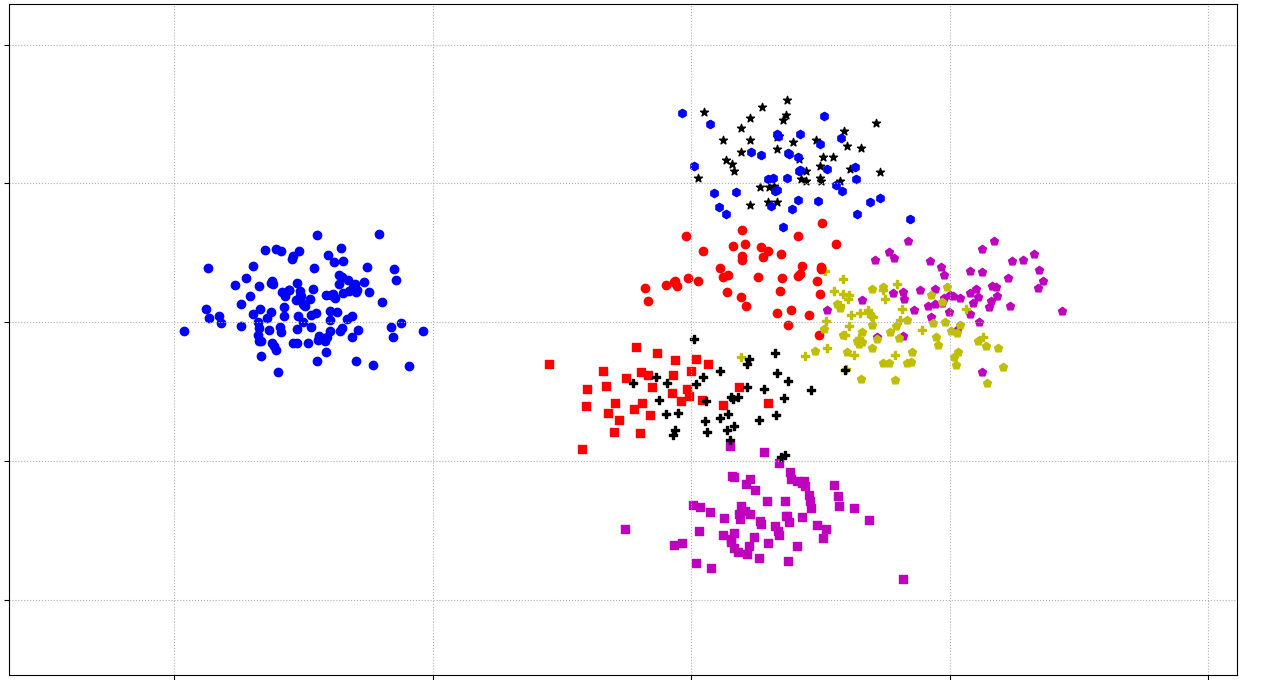
\includegraphics[width=0.49\textwidth]{img/svd-kovaleva-025}}
		\subfigure[a=0.50] {\label{fig:svd-gen2}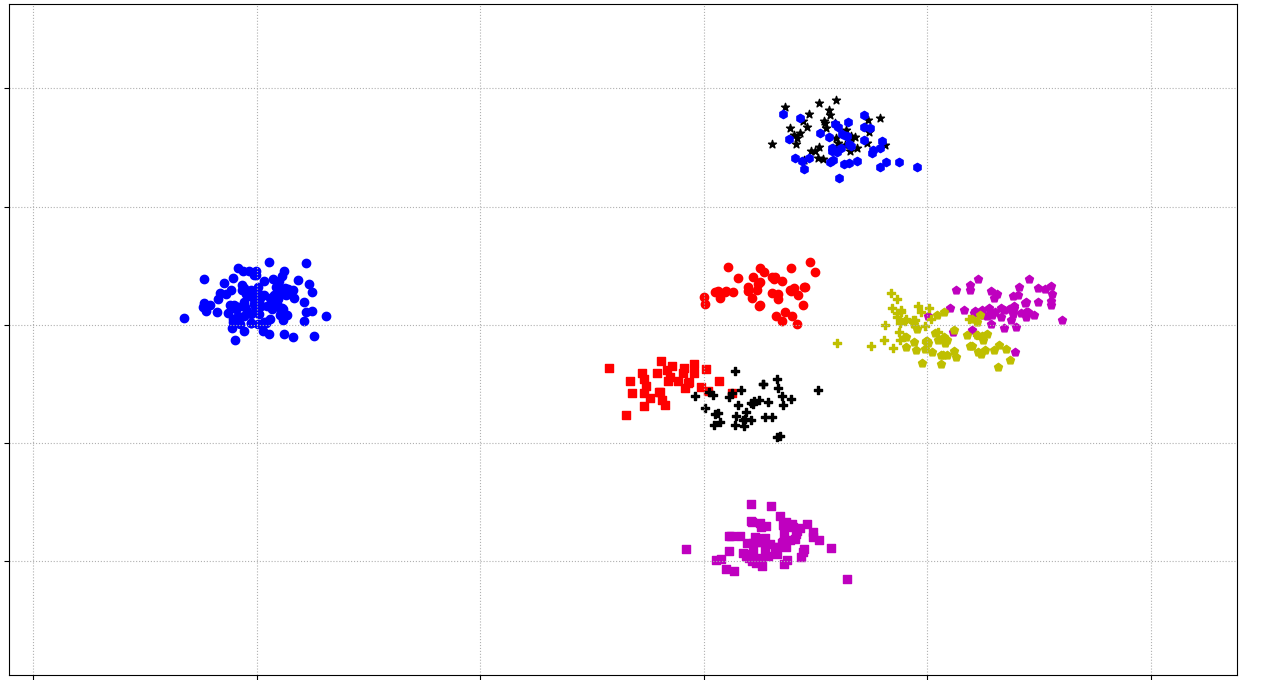
\includegraphics[width=0.49\textwidth]{img/svd-kovaleva-050}}
		\subfigure[a=0.75] {\label{fig:svd-gen3}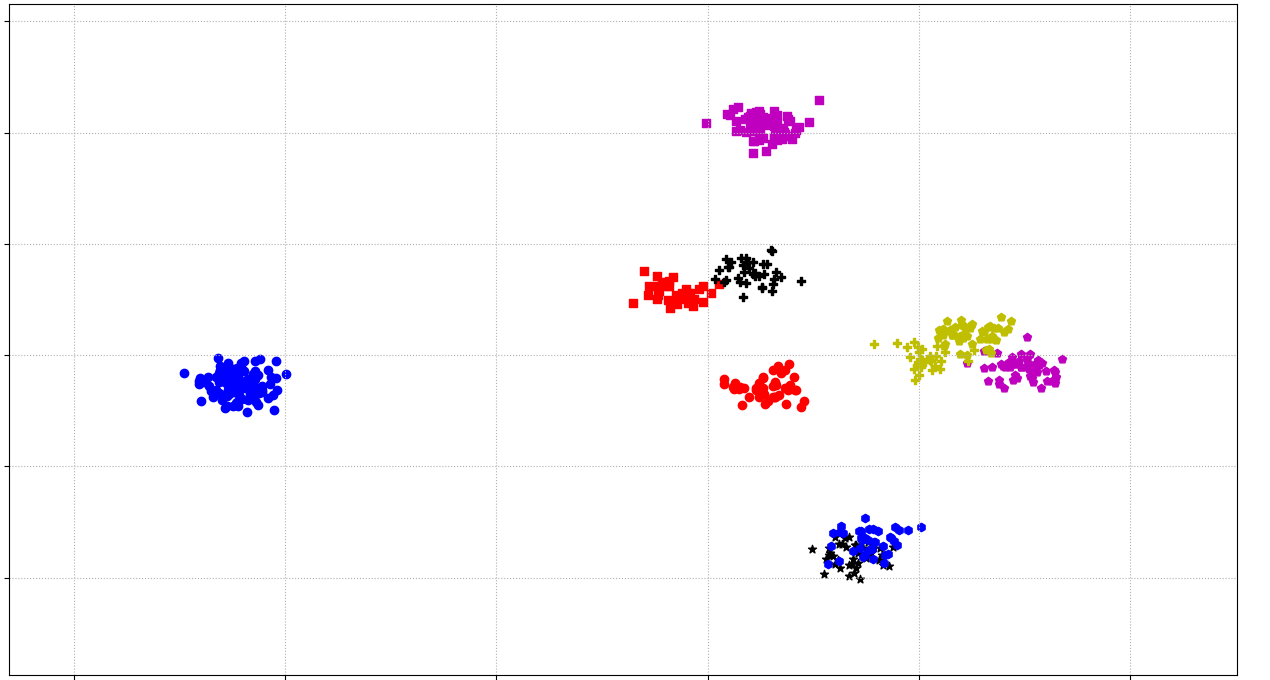
\includegraphics[width=0.49\textwidth]{img/svd-kovaleva-075}}
		
		\caption{Сгенерированные данные для трёх случаев параметра $ a $
			\\ {\small Для трёх значений параметра $ a = 0.25,\;0.50,\;0.75$ приведена диаграмма, изображающая проекции сгенерированных данных на главные компоненты. Данные сгенерированы при числе признаков, равным 10; общее число объектов --- 500; минимальная численность кластера --- 30.}}
		\label{fig:svd-gen}
	\end{figure}
	
	Структура получаемых данных представляет собой заданное количество гауссовых кластеров $ K $, сформированных при фиксированном общем числе объектов $ N $ и признаков $ V $ и заданным минимальным количестве объектов в каждом кластере $ m $. Остаток нераспределенных объектов $ \delta = N-K \cdot m $ размещается случайно и равномерно по всем кластерам. Для этого генерируется $ K-1 $ псевдослучайных числа в диапазоне от $ 0 $ до $ 1 $, к сгенерированным числам добавляется $ 0 $ и $ 1 $, после чего они упорядочиваются и вычисляется разность между соседними элементами в полученной последовательности. Эти разности определяют долю от нераспределенных объектов, которые будут дополнительно включены в $ K $ кластеров. Таким образом достигается строгое соблюдение общего числа объектов и равномерное распределение остатка по кластерам. 
	
	При определённой численности, кластер генерируется из многомерного распределения Гаусса. Среднее кластера выбирается случайно при равномерном распределении из множества $ [-a,a]^V $, где $ a \in [0,1] $ --- параметр, влияющий на взаимное смешивание кластеров: чем меньше $ a $, тем сложнее разделить сгенерированные кластеры. Ковариационная матрица формируется как диагональная с элементами, сгенерированными случайно из равномерного распределения в диапазоне $ [0.05\:a, 0.1\:a] $. 
	На рисунке показаны примеры сгенерированных данных 
	
	
	\subsection{Интерпретация результатов}
	
	В системе INDACT встроен модуль генерации отчётов, который позволяет пользователю получить основную информацию относительно каждого кластера и разбиения в целом. В данном разделе будут описаны математические зависимости, которые лежат в основе характеристик, используемых в отчёте. 
	
		
	\subsubsection{Оценка качества разбиений}
	
	При проведении кластер-анализа часто встаёт задача определения качества полученного разбиения. Например, вопрос о качестве разбиения может возникнуть при выборе наиболее подходящего алгоритма для анализируемых данных. В программе INDACT применяется две методики: индекс ARI и эмпирическая характеристика SW. Первая методика используется при сравнении разбиения с заданным эталонным. Эмпирическая характеристика SW не зависит от базового разбиения и может быть применена для одного разбиения при неизвестном эталонном. Однако, следует понимать, что SW не учитывает специфики предметной области и может в частных случаях давать искажённое представление о качестве разбиения. С другой стороны, на синтетических данных, для хорошо разделимых гауссовых кластеров, характеристика SW достаточно точно воспроизводит поведение индекса ARI относительно истинного разбиения, которое известно исходя из генерации кластеров.

	\subsubsection{Характеристика Silhouette Width}

	Эмпирическая характеристика Silhouette Width (SW) основывается на общем представлении о сильной близости внутри группы и хорошей разделимости кластеров. SW \cite{sw-canonical} принимает значения от -1 до 1 и для отдельного объекта вычисляется по следующей формуле:
	 \begin{equation*}
	 SW(y_i) = \dfrac{b(y_i)-a(y_i)}{max\{a(y_i),b(y_i))\}},
	 \end{equation*}
	 \begin{conditions}
	 	a(y_i) & среднее расстояние между объектом $ y_i \in C_k $ и всеми объектами,\newline     принадлежащими тому же кластеру $ C_k $, что и $ y_i $; \\
	 	b(y_i) & наименьшее среднее расстояние между объектом $ y_i \in C_k $ и объектами,\newline  которые принадлежат другим кластерам. \\
	 \end{conditions}
	 
	 Для разбиения характеристика SW определяется как среднее по всем объектам: $ SW(S) = \dfrac{1}{N} \sum_{k=1 }^{K} \sum_{i \in C_k}^{} SW(y_i) $. Значения, наиболее близкие к $ 1 $ соответствуют наилучшим разбиениям. Как показали эксперименты, характеристика SW ведёт себя примерно тем же образом что и широко известный индекс ARI \cite{ari-canonical}, который позволяет оценить качество разбиения, сравнивая его с истинным. 
	 
	
	\subsubsection{Adjusted Rand Index}
	
	Индекс ARI (Adjusted Rand Index) \cite{ari-canonical} является популярным способом сравнения эталонного и заданного разбиения. В условиях проводимого эксперимента используются синтетические данные, для которых известно истинное разбиение, поэтому для оценки эффективности применения эмпирической характеристики SW можно задействовать ARI. Формула для вычисления индекса записывается следующим образом:
	
	\begin{equation*} \label{eq:ari}
	ARI = \dfrac{\sum_{ij}\binom{n_{ij}}{2}-\left [ \sum_{i}\binom{a_{i}}{2}\sum_{j}\binom{b_{j}}{2} \right ]/\binom{n}{2}}{\dfrac{1}{2} \left [ \sum_i \binom{a_i}{2} + \sum_j \binom{b_j}{2} \right ] - \left [ \sum_i \binom{a_i}{2} \sum_j \binom{b_j}{2} \right ]/ \binom{n}{2}}
	\end{equation*}
	\begin{conditions}
		n_{ij} = |C_i \cap C_j|  & число объектов, входящий одновременно в $ i $-ый \newline  
		кластер в первом разбиении и в $ j $-ый --- во втором. \\
		a_{i} = \sum_{j=1}^{K} |C_i \cap C_j|  & число объектов, ходящих в $ i $-ый кластер в первом разбиении\\
		b_{j} = \sum_{i=1}^{K} |C_i \cap C_j|  & число объектов, ходящих в $ j $-ый кластер во втором разбиении\\
	\end{conditions}
	
	Как и характеристика SW, индекс ARI принимает значения от -1 до 1. ARI достигает 1 только в том случае, если два разбиения совпадают.
	
	\subsubsection{Характеризация кластеров}
	По каждому полученному кластеру $ C_k $ в отчёте INDACT приводится его центр, вычисленный для каждого признака как среднее по всем объектам кластера:
	
	\begin{equation*} 
	c_{kv} = \frac{1}{|C_k|} \sum_{i \in C_k}^{} y_{iv}
	\end{equation*}
	
	Центр кластера может вычисляться как по нормализованным, так и по исходным признакам. Для исходных признаков часто полезно знать разницу между глобальным центром данных и среднем по кластеру, как в абсолютном выражении, так и в процентном:
	
	\vspace*{1\baselineskip} 
	\noindent\begin{minipage}{.5\linewidth}
		\begin{equation*}
		D_{kv} = c_{kv} - \frac{1}{N} \sum_{i=1}^{N} y_{iv}
		\end{equation*}
	\end{minipage}%
	\begin{minipage}{.5\linewidth}
		\begin{equation*}
		D_{kv},\% = \frac{D_{kv}}{1/N \sum_{i=1}^{N} y_{iv}} \cdot 100 \% 
		\end{equation*}
	\end{minipage}%
	\vspace*{1\baselineskip} 

	Значимость кластера описывается его вкладом в квадратичный разброс данных. Квадратичный разброс данных и вклад в него заданного кластера $ C_k $ вычисляется по формулам, приведённым ниже:
	
	
	\vspace*{1\baselineskip} 
	\noindent\begin{minipage}{.5\linewidth}
		\begin{equation*}
		T(Y) = \sum_{i=1}^{N} y_{iv}^2
		\end{equation*}
	\end{minipage}%
	\begin{minipage}{.5\linewidth}
		\begin{equation*}
		contrib_k,\% =  |C_k| \frac{<c_{k},c_{k}> }{T(Y)}\cdot 100\%
		\end{equation*}
	\end{minipage}%
	\vspace*{1\baselineskip} 
	
	Общий вклад кластеров в квадратичный разброс данных может быть получен суммированием вклада по каждому из кластеров: $ contrib,\% = \sum_{k=1}^{K} contrib_k,\% $. Для того чтобы лучше понять что из себя представляют кластеры, в отчёте для каждого кластера отмечаются и выписываются признаки, которые превосходят по относительной разности заданный порог $ \Theta_D $. 	По-умолчанию пороговое значение выставлено равным $ 30\% $. Таким образом, в заданном кластере $ C_k $ признаки условно разделяются на:
	\begin{itemize}
		\item большие: $ \{v: D_{kv},\% > \Theta_D\} $
		\item маленькие: $ \{v: -D_{kv},\% > \Theta_D\} $
	\end{itemize}

	Вклад каждого кластера в квадратичный разброс данный может быть расписан по каждому признаку отдельно. Для определения вклада признака $ v $ в квадратичный разброс данных внутри кластера $ C_k $ применяется следующая формула:
	
	\begin{equation*}
	contrib_{kv},\% = |C_k| \frac{c_{kv}^2}{T(Y)} \cdot 100\%
	\end{equation*}	
	
	Сумма вклада $ contrib_{kv},\%  $ по всем признаком внутри кластера $ C_k $ равна общему вкладу этого кластера в разброс данных: $\sum_{v=1}^{V} contrib_{kv},\%  = contrib_{k},\%  $. Для вычисления относительного вклада вычисляется вклад каждого признака $ v $ без учёта разбиения $ contrib_v $ и определятся отношение вклада внутри кластера $ contrib_{kv},\%  $  к $ contrib_v $.
	
	\vspace*{1\baselineskip} 
	\noindent\begin{minipage}{.5\linewidth}
		\begin{equation*}
		contrib_v,\% = \frac{\sum_{i=1}^{N} y_{iv}^2}{T(Y)}			
		\end{equation*}
	\end{minipage}%
	\begin{minipage}{.5\linewidth}
		\begin{equation*}
		contrib_{kv}^{relative} = \frac{contrib_{kv}}{ contrib_v}
		\end{equation*}
	\end{minipage}%
	\vspace*{1\baselineskip} 
	
	\subsection{Общие рекомендации по выбору алгоритма}
	
	В разделах \ref{subsec:anomalous}---\ref{subsec:bikmr} описаны алгоритмы, реализованные программной системой INDACT. Полный  перечень алгоритмов, которые можно применить к данным, представлен ниже:
	
	\begin{enumerate}
		\item \ikmeans
		\item \AWard
		\item \AWardpb
		\item \dePDDP
		\item \BiKMR
	\end{enumerate}
	
	
	Алгоритмы \ikmeans, \dePDDP, \BiKMR находят число кластеров автоматически, причём по-умолчанию в них используются определённые значения параметров, выбор которых определяет число получаемых кластеров. В \ikmeans по-умолчанию задан порог $ \Theta=1 $ минимального числа объектов в аномальной группе, в алгоритме \dePDDP задействована величина ``окна Парзена'' $ h $, определяемая как указано в пояснениях к формуле \eqref{eq:parzen}, а в \BiKMR предопределена доля некорректных направлений $ \epsilon=0,32 $. Значения параметров в \dePDDP и \BiKMR найдены  экспериментально и, как правило, не требуют регулировки. Значение параметра в \ikmeans $ \Theta=1 $ обычно приводит к избыточному числу кластеров, что лежит в основе алгоритмов \AWard и \AWardpb, которые начинают именно с этих кластеров и последовательно их объединяют. При этом алгоритм \AWardpb включает два параметра, настраиваемых вручную. Его использование рекомендуется только в случае, когда ожидается, что признаки слабо соответствуют искомой кластерной структуре. Нормально, пользователю следует начать с алгоритма \ikmeans и применять \AWard для последовательного объединения полученных кластеров, если \ikmeans дал слишком большое число кластеров. Если ожидается, что в данных много случайных, нехарактерных объектов, то лучше применять метод \BiKMR.
	
	\section{Пользовательское описание программы INDACT}
	
	С точки зрения пользователя программная система INDACT представляет собой оконное приложение с графическим интерфейсом, в целом аналогичным интерфейсу большинства современных программ. Программа имеет одно основное окно, в котором одновременно отображаются и обрабатываемые и нормализованные данные, а также множество вспомогательных и диалоговых окон, возникающие в результате взаимодействия с пользователем. 
	
	INDACT распространяется в виде каталога бинарных файлов, который содержит все необходимые библиотеки уже скомпилированные для операционной системы, поэтому от пользователя не требуется устанавливать никакие дополнительные компоненты (в том числе интерпретаторы или модули).
	
	В данном разделе продемонстрированы основные элементы интерфейса, а также некоторые диалоговые окна. Подробнее все функции системы описаны в руководстве пользователя. Также в руководстве пользователя предметно указаны требования к характеристикам персонального компьютера (ПК) и программному обеспечению, однако, кратко отметим, что INDACT работает практически на всех современных ПК под управлением Microsoft Windows 7 и выше. 
	
	\subsection{Этапы работы с программой}
	
	Работа с программой в типичном случае состоит из четырёх базовых этапов, которые пользователь проходит последовательно  как изображено на рисунке \ref{fig:stages}. Тем не менее, это не означает что указанная последовательность жёстко фиксирована и нет возможности вернуться на предыдущий этап. Если пользователь допустил ошибку или намерен опробовать различные варианты, он может заново вызвать функции с произвольного предыдущего этапа.
	\vspace*{1\baselineskip} 
	\begin{figure}[h!]
		\centering		
		\includestandalone[width=\linewidth]{tikz/stages}
		\caption{Основные этапы работы с программой}
		\label{fig:stages}
	\end{figure}
	
	На этапе загрузки данных пользователь должен выбрать текстовый файл с данными и загрузить его в программу. Текстовый файл представляет собой таблицу данных, каждая строка которой соответствует строке файла, а столбцы разделены запятыми. После загрузки файла графический интерфейс отобразит загруженные данные и они станут доступны для работы. Единовременно программой предусмотрена работа только с одним файлом.
	
	Нормализация является подготовительным этапом, тем не менее, этот этап очень важен для успешной работы алгоритмов кластеризации. В диалоговом окне доступен выбор параметров нормализации описанных в разделе \ref{subsec:normalization}. Программа INDACT допускает изменение настроек нормализации практически на любом этапе обработки данных. В рамках нормализации в программной системе также рассматривается отбор признаков, которые будут участвовать в кластеризации. При отборе также решается вопрос о включении номинальных признаков, которые автоматически разбиваются на бинарные, после чего нормируются в соответствии с заданными настройками.
	
	Этап кластеризации состоит в выборе подходящего алгоритма, задания параметров (при необходимости) и его выполнении. После выполнения алгоритма становится известно разбиение, которое ставит в соответствие каждому объекту номер кластера, которому объект принадлежит. Программа INDACT допускает работу одновременно с несколькими разбиениями. Таким образом, можно получить несколько различных результатов для разных значений параметров или алгоритмов и после этого приступить к анализу, выбрав наиболее подходящее разбиение. 
	
	Анализ результатов заключается в оценке полученных разбиений а также интерпретации кластеров. Для этого используется модуль генерации отчёта. Результирующий отчёт, нормированные и исходные признаки, а также признак, определяющий кластерную принадлежность объектов можно сохранить в текстовый файл. Кроме того, в рамках анализа функционалом системы предусмотрена возможность построения поля рассеивания по указанным признакам, а также  SVD диаграммы с цветовым выделением кластеров и гистограммы заданного признака.
	
	\subsection{Основные сведения о пользовательском интерфейсе}
	
	Главное окно программы INDACT (см. рисунок \ref{fig:main-gui}) содержит главное меню (1), панель  управляющих кнопок (2) и две таблицы: исходных (3) и нормализованных данных~(4) . 
	\begin{figure}[h!]
		\centering
		\includestandalone[width=0.8\linewidth]{tikz/main-gui}				
		\caption{Главное окно программы INDACT}
		\label{fig:main-gui}
	\end{figure}
	\newpage
	Главное меню содержит большинство операций программы и имеет структуру вложенных подменю как показано на рисунке \ref{fig:menu}. 
	\begin{figure}[h!]
		\centering
		\includestandalone[width=\linewidth]{tikz/menu}				
		\caption{Структура главного меню}
		\label{fig:menu}
	\end{figure}
	
	Меню File содержит основные операции, такие как загрузка файла данных, операции с данными, сохранение данных и выход из программы. Операции с данными включают одновременную нормализацию нескольких признаков, очистку панели нормализованных данных и генерацию синтетических данных. 
	
	Пункт меню Run предоставляет пользователю возможность выбора одного из 5 реализованных алгоритмов. При выборе пункта меню, соответствующего алгоритму, при необходимости откроется окно ввода параметров алгоритма (некоторые алгоритмы, например, \dePDDP, не требуют настройки), через которое осуществляется запуск на выполнение.
	
	Меню Plot содержит базовые операции для графического представления данных. Например, у пользователя есть возможность присвоить признакам маркеры X и Y, определяющие признак, который будет отложен по оси абсцисс и ординат соответственно при построении поля рассеивания. Также пользователь может оценить общую структуру многомерных данных при помощи SVD диаграммы. 
	
	Для генерации отчёта предназначен пункт главного меню Report. Этот пункт содержит два действия для построения текстового отчёта и отчёта по центрам кластеров.
	
	Вызов некоторых команд осуществляется с панели управляющих кнопок. Предусмотрены управляющие кнопки для следующих действий:
	\begin{itemize}
		\item 
\includegraphics[scale=0.05]{img/folder-ico} загрузить файл
		\item 
\includegraphics[scale=0.1]{img/settings} настройки нормализации
		\item 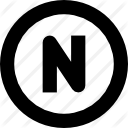
\includegraphics[scale=0.05]{img/norm} вкл./выкл. нормализацию
		\item 
\includegraphics[scale=0.1]{img/norm_all} нормализовать выбранные признаки
		\item 
\includegraphics[scale=0.1]{img/delete} удалить выбранные признаки
		\item 
\includegraphics[scale=0.1]{img/clustering} отобразить/скрыть раздел результатов
	\end{itemize}
	
	\subsection{Загрузка данных}
	
	Загрузка данных --- начальный этап работы с программой. Для того чтобы указать программе из какого файла следует извлечь данные, пользователь выполняет процедуру загрузки текстового файла. Загружаемый файл должен отвечать определенным требованиям, в частности, каждая строка файла соответствует одному объекту и значения признаков разделены запятой. Расширение имени файла при загрузке во внимание не принимается, однако важно чтобы файл быть текстовым, а не бинарным. Подробно требования к файлу описаны в руководстве пользователя. 
	
	Для загрузки файла пользователь выбирает меню File \textrightarrow Load data file. Это действие приводит к открытию стандартного диалога загрузки файла. Того же эффекта можно добиться нажатием иконки 
\includegraphics[scale=0.05]{img/folder-ico} на управляющей панели.
	
	На рисунке \ref{fig:load-dialog} показан диалог загрузки в операционной системе Windows. Пользователь должен проследовать в файловом диалоге по пути к загружаемому файлу и выделить его, после чего подтвердить выбор.

	\begin{figure}[h!]
		\centering
		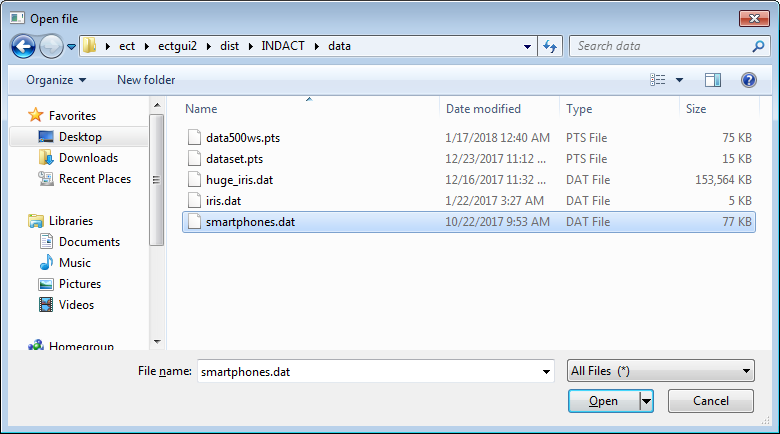
\includegraphics[width=0.8\linewidth]{img/instruction/open-smartphones}
		\caption{Диалог загрузки данных}
		\label{fig:load-dialog}
	\end{figure}
	
	Загруженные данные отображаются в программе в таблице исходных данных. Пользователю следует убедиться, что загружен правильный файл, объекты и признаки отображаются верно. После успешной загрузки пользователь может начинать отбор признаков и их нормализацию.
	
	\subsection{Генерация синтетических данных}

	Генерация данных включена в состав системы для проведения численных экспериментов. Используется метод генерации, описанный в разделе \ref{subsec:generator}, который позволяет зафиксировать наиболее значимые характеристики кластерной структуры.
	
	Чтобы запустить модуль генерации данных, пользователь выбирает пункты меню File \textrightarrow Data operations  \textrightarrow Generate. Диалоговое окно генератора данных, показанное на рисунке \ref{fig:generator-dialog}, позволяет ввести значения характеристик в текстовые поля в нижнем правом углу окна. Сразу же после ввода будет обновлена SVD диаграмма сгенерированных данных. Таким образом, пользователь может непосредственно оценивать влияние изменения параметра и подбирать  значения, наиболее подходящие для его задачи.
			
	Окно генератора требует ввода следующих 6 числовых параметров:
	\begin{itemize}
		\item Seed generation --- начальная установка генератора случайных чисел, служит для обеспечения повторяемости результата;
		\item Minimum cluster cardinality --- минимальное число объектов в каждом кластере;
		\item Number of clusters --- число генерируемых кластеров;
		\item Number of objects --- число объектов, распределяемых по кластерам;
		\item Features --- количество признаков;
		\item Box parameter (a) --- параметр, определяющий степень взаимного смешивания кластеров, чем больше значение, тем легче разделить сгенерированные кластеры.
	\end{itemize}
	
	\begin{figure}[h!]
		\centering
		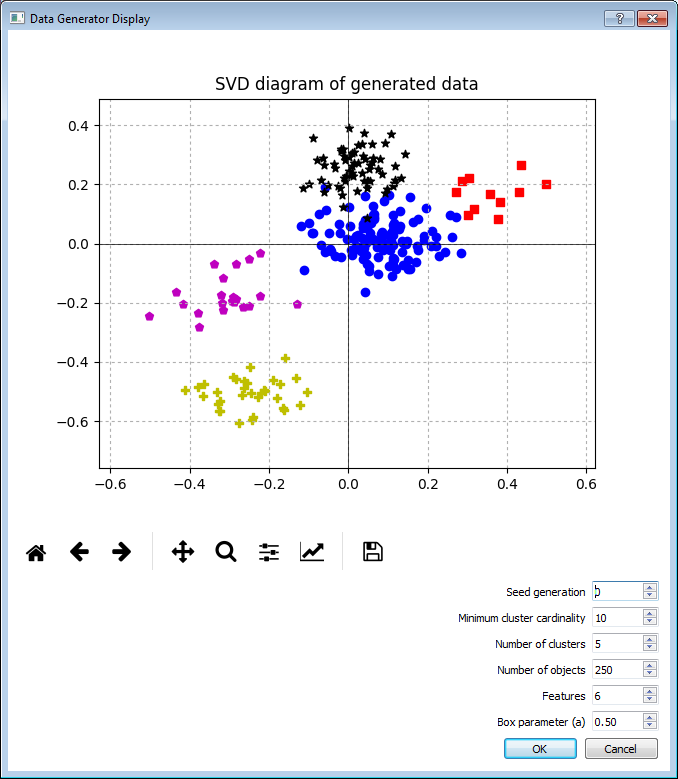
\includegraphics[width=0.7\linewidth]{img/instruction/gen-data-dialog}
		\caption{Диалог генератора данных}
		\label{fig:generator-dialog}
	\end{figure}
	
	После подтверждения ввода пользователю будет предложено выбрать путь для сохранения сгенерированных данных, а также выбрать способ сохранения признака, обозначающего кластерную принадлежность объекта. Этот признак можно сохранить в тот же файл, в котором содержатся сгенерированные данные в качестве отдельного столбца или сохранить его в другом текстовом файле.
	
	\subsection{Нормализация данных}
	
	Нормализация данных осуществляется в два этапа. На первом этапе происходит настройка параметров: способа преобразования начала отчёта и масштаба. Второй этап заключается в выборе признаков, которые будут участвовать в кластеризации. Для этого требуется перенести соответствующие признаки на панель нормализованных данных. Чтобы нормализовать отдельный признак, в контекстном меню следует выбрать пункт Normalize. Если необходимо нормализовать сразу группу признаков, удобнее воспользоваться кнопкой 
\includegraphics[scale=0.1]{img/norm_all}, что позволит отметить для нормализации сразу несколько признаков. Изменить настройки нормализации можно нажав кнопку 
\includegraphics[scale=0.1]{img/settings}. При этом новые настройки применяются как для тех признаков, которые уже находятся в области нормализованных, так и для вновь нормализуемых. Окно настройки параметров показано на рисунке \ref{fig:norm-dialog}. В качестве справочной информации в это окно встроена основная формула нормализации \eqref{eq:data-Y}. Отдельным флажком Normalization enabled переключается текущее состояние: вкл./выкл. Если нормализация выключена, то все выбранные признаки будут использованы в том виде, в котором они были загружены из файла.
	
	\begin{figure}[h!]
		\centering
		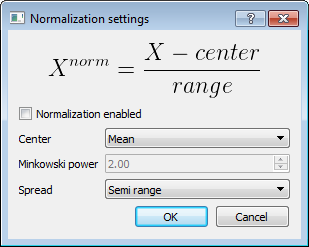
\includegraphics[width=0.35\linewidth]{img/instruction/norm-dialog}
		\caption{Диалог настройки нормализации}
		\label{fig:norm-dialog}
	\end{figure}
	
	Для задания параметров нормализации доступны следующие значения:
	\begin{flushleft}
		\begin{tabular}{ l l }
			Center: & Mean: \\
			\tabitem No centring &	\tabitem Unity \\
			\tabitem Mean &	\tabitem Semi range \\
			\tabitem Minimum &	\tabitem Standard deviation \\
			\tabitem Median &	\tabitem Absolute deviation \\
			\tabitem Minkowski center &	 \\						
		\end{tabular}
	\end{flushleft}
	
	Текстовое поле Minkowski power становится активно только в том случае, если для центрирования выбрано значение ``Minkowski center''. Нормализованные данные отображаются в правой панели, как показано на рисунке \ref{fig:norm-data}.
	
	\begin{figure}[h!]
		\centering
		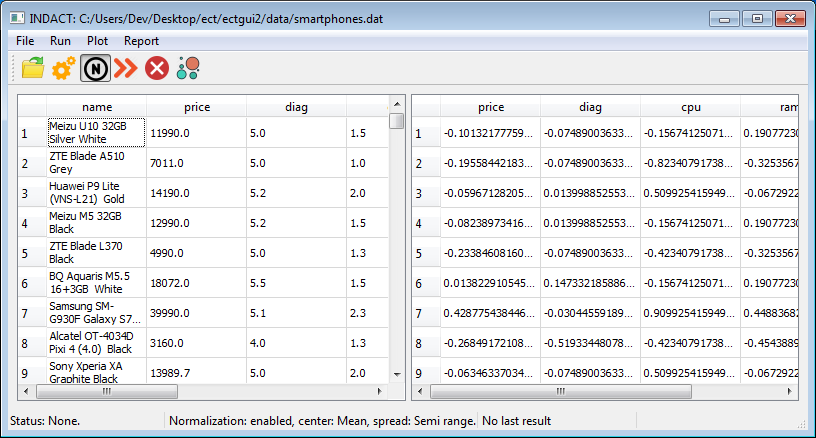
\includegraphics[width=0.8\linewidth]{img/main-gui.png}				
		\caption{Отображение нормализованных данных}
		\label{fig:norm-data}
	\end{figure}
	
	\subsection{Кластеризация}\label{subsec:clustering}
	Нормализованные данные готовы для выполнения алгоритма кластеризации. Для получения кластерного разбиения требуется выбрать один из алгоритмов кластеризации из меню Run. Каждый алгоритм, за исключением \dePDDP обладает своим окном настроек параметров. Окна настроек параметров алгоритмов приведены на рисунке \ref{fig:alg-dialogs}. Для получения более подробной информации относительно настройки параметров в диалоговых окнах следует обратиться к руководству пользователя.
	
	\begin{figure}[h!] % \ContinuedFloat
		\begin{subfigmatrix}{2}
		\centering
		\subfigure[\ikmeans] {\label{fig:ikmeans}\raisebox{2mm}{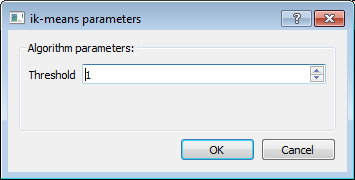
\includegraphics[width=0.45\textwidth]{img/instruction/param-dialog-ikmeans}}}
		\subfigure[\AWard] {\label{fig:award}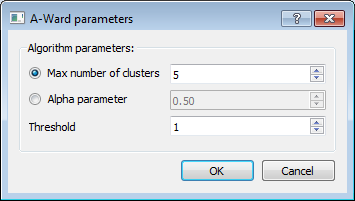
\includegraphics[width=0.45\textwidth]{img/instruction/param-dialog-a-ward}}
		\subfigure[\AWardpb] {\label{fig:awardpb}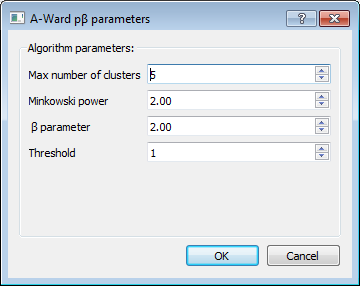
\includegraphics[width=0.45\textwidth]{img/instruction/param-dialog-a-ward-pb}}
		\subfigure[\BiKMR] {\label{fig:bikmr}\raisebox{10mm}{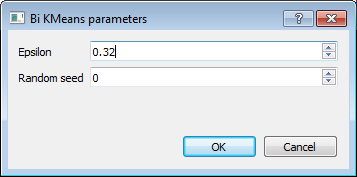
\includegraphics[width=0.45\textwidth]{img/instruction/param-dialog-bikmr}}}
	\end{subfigmatrix}
		\caption{Диалоговые окна для задания параметров алгоритмов}
		\label{fig:alg-dialogs}
	\end{figure}
	
	После ввода необходимых параметров и подтверждения ввода запускается алгоритм кластеризации. На относительно небольших данных (до 500 объектов) кластеризация обычно не занимает более 20--30 сек. При успешной отработке алгоритма автоматически откроется дополнительная панель результатов. Благодаря этой панели имеется возможность хранить сразу несколько разбиений, переключаясь между ними чтобы исследовать свойства каждого из них. На рисунке \ref{fig:clustering-result} приведён вид окна с открытой панелью результатов после однократного запуска \dePDDP. Как можно видеть на этом рисунке, панель содержит столбец \texttt{dePDDP\_1}, который отображает соответствие каждого объекта одному из сформированных кластеров, используя для этого его номер.
	
	\begin{figure}[h!]
		\centering
		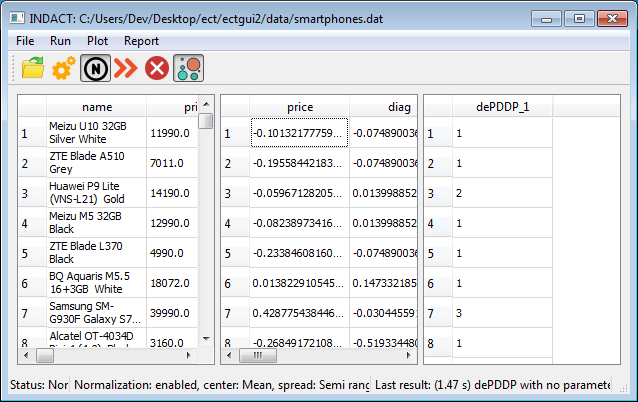
\includegraphics[width=0.8\linewidth]{img/clustering-result}		
		\caption{Отображение результата кластеризации}
		\label{fig:clustering-result}
	\end{figure}
	
	Примечательно, что результат кластеризации может быть получен и косвенным образом. Например, данные уже содержат признак, который определяет разбиение на множестве объектов. В таком случае этот признак можно занести в панель результатов из контекстного меню, выбрав пункт To labels. Этот результат будет обладать тем же функционалом для анализа, что и результаты, полученные путём выполнения алгоритма кластеризации. Таким образом, программа может быть использована как средство анализа результата, полученного сторонними средствами и сохранённым в текстовом файле.
	
	\subsection{Анализ результатов}
	Для анализа результатов программой INDACT генерируется настраиваемый текстовый отчёт. В отчёт включены основные характеристики кластеров и разбиения в целом, в том числе оценки качества. Для вывода диалогового окна (рисунок \ref{fig:report-dialog}) с текстовым отчётом требуется в главном меню выбрать пункты Report \textrightarrow Report table. При перед открытием окна у пользователя будет возможность выбрать то, разбиение относительно которого требуется провести анализ. Как было упомянуто выше в разделе \ref{subsec:clustering}, программа может одновременно хранить несколько разбиений, однако в момент построения отчёта требуется указать одно из доступных.
	
	\begin{figure}[h!]
		\centering
		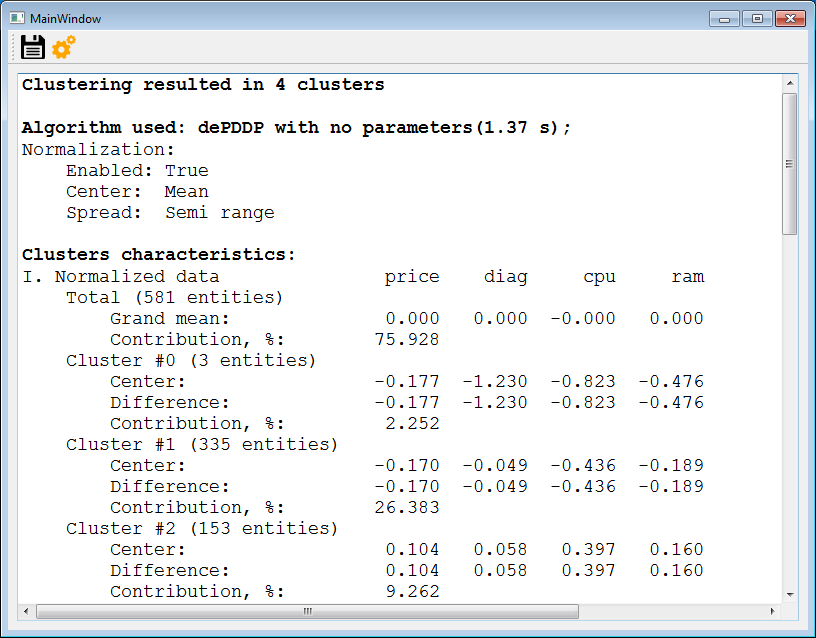
\includegraphics[width=0.7\linewidth]{img/report-dialog}		
		\caption{Диалоговое окно отчёта}
		\label{fig:report-dialog}
	\end{figure}
	
	Общая структура отчёта представлена ниже:
	
	\begin{itemize}
		\item Число полученных кластеров
		\item Применённый алгоритм с указанием параметров
		\item Используемые настройки нормализации
		\item (Опционально) Оценка разбиений: SW, ARI.
		\item Характеристика кластеров в нормализованных признаках
		\item Характеристика кластеров в исходных признаках
		\item Перечень отличительных признаков кластеров
		\item Таблица вклада каждого кластера в квадратичный разброс данных по признакам
		\item Таблица вклада каждого признака в квадратичный разброс без учёта кластеризации
		\item Таблица относительного вклада каждого кластера в квадратичный разброс данных по признакам
		\item (Опционально) Таблица сопряженности
		\item (Опционально) Перечень объектов заданных кластеров
	\end{itemize}
	
	По-умолчанию в отчёт не включаются величины, вычисление которых может занять продолжительное время. Например, к таким величинам относятся характеристики разбиений SW и ARI. Включить вычисление этих характеристик а также задать эталонное разбиение можно при помощи диалогового окна настроек, которое вызывается нажатием кнопки 
\includegraphics[scale=0.1]{img/settings} в окне отчёта. Когда отчёт сформирован надлежащим образом, пользователь может сохранить его в текстовый файл при помощи кнопки 
\includegraphics[scale=0.1]{img/save}.
	
	Также к этапу анализа можно отнести построение SVD диаграммы, поля рассеивания и гистограммы. SVD диаграмма может быть построена при помощи выбора в главном меню пункта Plot \textrightarrow SVD. Для построения поля рассеивания от пользователя требуется предварительно выставить так называемые метки, которые определяют роль признака. Метка \texttt{X} задаёт признак по оси абсцисс, а метка \texttt{Y} --- по оси ординат. Задание меток осуществляется из контекстного меню соответствующего признака (подробнее см. руководство пользователя). Функция построения гистограммы также входит в контекстное меню признака.
	
	\section{Структурное описание программы INDACT} \label{sec:structure}
	
	В данном разделе рассматриваются технические особенности системы INDACT. Перед разработчиком стоит задача написать программу, реализующую сложные алгоритмы вычислений и предоставить пользователю удобный и современный графический интерфейс. При этом желательно, чтобы требования к конфигурации ПК, на котором будет запускаться программы были как можно менее строгими. 
	
	Для решения этой задачи потребуется аккуратный выбор программных средств, таких как язык программирования и программные библиотеки. От выбора программных средств во многом зависит трудоёмкость создания продукта и его некоторые потребительские качества, например, кросплатформенность и необходимость установки дополнительных компонент. Кроме того удачный выбор используемых программных библиотек позволит существенно сократить объем вновь разрабатываемого кода, что положительно скажется на отказоустойчивости продукта и уменьшит  возможность возникновения ошибок. 
	
	\subsection{Выбор методологии разработки}
	Разработка программных систем осуществляется как правило в рамках какой-либо методологии. Методология определяет общую концепцию организации работ, роль заказчика в процессе разработки, порядок внесения изменений и выпуска версий. Конечно, преимущества различных методологий в основном заметны при работе над крупными и затратными проектами, которые требуют координации усилий больших коллективов специалистов. Тем не менее, даже при разработке относительно несложных программ полезно придерживаться определённой дисциплины в организации работ, что позволит написать структурированный код, пригодный к поддержке на протяжении долгого времени.
	
	В настоящее время наиболее популярны методологии Agile, TDD, RAD и другие. Гибкая методология Agile ориентирована на динамическое формирование требований и итеративную разработку. Говорить о методологии  Agile целесообразно в том случае, если над программным продуктом трудится несколько небольших групп разработчиков. В начале 2000-ых появилась и начала интенсивно развиваться методология разработки через тестирование (test-driven development TDD), которая в некоторой степени является противоположностью Agile. В ней подразумевается написание тестов до того как будет готов тестируемый программный код, соответственно требования должны быть известны заранее. При аккуратном следовании методологии TDD разработанный продукт отличается высоким качеством и устойчивостью к сбоям, однако затраты на написание тестов могут существенным образом замедлить разработку. В условиях сжатых сроков при небольшой стоимости продукта наиболее эффективно показала себя методология быстрой разработки приложений RAD (rapid application develompent). RAD основана на инкрементальном прототипировании и широком применении средств визуального проектирования. Как и в случае c Agile, RAD позволяет изменять требования к системе по мере выработки мнения заказчика относительно того или иного технического решения. В целом RAD отвечает ограничениям, которые следует принять во внимания при разработке INDACT: необходимо выполнить проект в сжатые сроки; изначально требования к программе определены  нечетко, возможно их изменение; проект выполняется без финансирования; графическому интерфейсу пользователя отводится важная роль.

	\subsection{Выбор программных средств}
	
	\subsubsection{Язык программирования} 
	Выбору языка программирования следует уделить большое внимание. В настоящее время для решения различных задач программисту доступен широкий выбор языков программирования. Существующие языки программирования
	сильно различаются по возможностям, гибкости и области применения. Многие языки, ранее считавшиеся передовыми, в наше время практически не применяются, так как они были вытеснены более современными. Сразу ограничимся наиболее распространёнными языками, что позволит, в случае необходимости, производить доработку программы разными программистами. 
	
	Аналитическая фирма RedMonk регулярно отслеживает тенденции в области информационных технологий и публикует рейтинг языков программирования. Рейтинг составляется с учётом числа заданных вопросов на известном информационном ресурсе \href{https://stackoverflow.com/}{stackoverflow.com} и количестве проектов, загруженных на хостинг \href{https://github.com/}{github.com}. Указанные ресурсы пользуются большой популярностью в информационном сообществе и рейтинг, составленный таким образом, вполне подходит для оценки популярности языков программирования. Согласно рейтингу RedMonk за 2018 год \cite{RedMonk}, наиболее распространены следующие языки:
	\begin{enumerate}
		\item JavaScript
		\item Java
		\item Python
		\item PHP
		\item C\#
		\item C++
	\end{enumerate}
	
	Исключим из приведённого перечня JavaScript и PHP, которые востребованы в большей степени для разработки веб-проектов. Таким образом, язык программирования для решения поставленной задачи будем выбирать из Java, Python, C\#, C++. Каждый из этих языков отличают свои особенности. 
	
	Java --- строго типизированный язык с автоматической сборкой мусора, применяется для серверных и корпоративных приложений. Java имеет широкую поддержку, как с точки зрения всевозможных справочных ресурсов, так и с точки зрения реализованных прикладных библиотек с открытым исходным кодом. К недостаткам языка можно отнести в некоторой степени избыточную по современным меркам ``многословность''. Возможно, этот недостаток проистекает из строгой типизации. С другой стороны, строгая типизация выступает преимуществом в той сфере, в которой как раз и применяется Java наиболее интенсивно --- для написания ответственных компонент распределённых приложений. Это позволяет отсеять многие ошибки ещё на этапе компиляции программы. 
	
	
	Набирающий популярность Python имеет большое число почитателей среди специалистов по анализу данных. С одной стороны, этот язык позволяет разработчику использовать традиционные подходы и конструкции, например, объектно-ориентированное программирование и классы. С другой стороны, в языке имеются чрезвычайно гибкие структуры, которые характерны для скриптовых языков. Динамическая типизация избавляет программиста от необходимости при объявлении каждый раз указывать тип переменных и в общем облегчает процедуру разработки. Также на языке реализованы многие удобные библиотеки обработки и анализа данных.
	
	Относительно C\# можно сказать, что в целом концептуально он не сильно отличается от Java. Однако, отдельно следует отметить следующую особенность: C\# разработан корпорацией Microsoft, поэтому о выполнении кода C\# на различных платформах (Linux, Mac) приходится размышлять только в теоретическом плане. На практике не существует официальных сред выполнения C\# кода для операционных систем за исключением Windows.
	
	С помощью C++ можно решить, как правило, любую задачу, однако это не означает что он одинаково удобен и для системного программирования и для написания небольшой программы с графическим интерфейсом. В C++ отсутствует автоматическая сборка мусора, выделение и освобождение памяти осуществляется в ручном режиме. Это обстоятельство может создавать большие неудобства. Если программист не будет аккуратно следить за выделяемой памятью, произойдёт ``утечка'' памяти и программа может завершиться аварийным выходом. Это лишь один аспект из многих, который следует учитывать при программировании на C++. Таким образом, при использовании C++ снижается скорость разработки, повышается трудоёмкость отладки и от программиста требуется наличие определённых навыков.
	
	По результатам проведённого анализа было принято решение сделать выбор в пользу Python. Многие возможности, обеспечиваемые языком Python, такие как лексические замыкания, значения параметров по умолчанию, неявная динамическая типизация и автоматическая сборка мусора, ускоряют разработку и позволяют сконцентрироваться непосредственно на реализуемом алгоритме. В то же время существует множество функциональных и хорошо документированных программных библиотек для Python. Наиболее известные из них --- NumPy для работы с многомерными массивами, Pandas для преобразования табличных данных и SciPy для научных вычислений.
	
	Для выполнения программы, написанной на Python происходит трансляция каждой инструкции в промежуточную форму --- байт-код. Байт-код выполняется в виртуальной машине Python. Виртуальные машины написаны для различных операционных систем, тем самым достигается независимость разработанного Python кода от используемой платформы. При этом несколько страдает производительность, но этот вопрос нельзя однозначно закрыть в пользу языков, компилируемых в машинный код, ведь виртуальная машина может оптимизировать как выделение памяти, так и выполнение различных инструкций. 
	
	\subsubsection{Библиотека графического интерфейса}
	Разработка программ с графическим пользовательским интерфейсом сильно упрощается при использовании готовых библиотек. Как правило, такие библиотеки позволяют создавать оконные приложения, на которых размещаются типовые элементы интерфейса: кнопки, переключатели, надписи и т.п. Практически все библиотеки предоставляют некоторый достаточный набор таких элементов, привычных пользователю современных операционных систем, некоторые библиотеки удобны для разработки собственных элементов управления. Поэтому при выборе библиотеки графического интерфейса будем руководствоваться в основном такими критериями, как удобство разработки, доступность справочной информации, кросплатформенность. Для Python наиболее распространены следующие библиотеки: Tkinter, wxPython, PyQt. Примеры окон приложений, отрисованных каждой из указанных библиотек в операционной системе Windows 7 приведены для сравнения на рисунке \ref{fig:gui-samples}. Как показал анализ с учётом рекомендаций на тематических ресурсах, наиболее сбалансированным решением представляется PyQt. 
	
	\begin{figure}[h!] % \ContinuedFloat
		\centering
		\begin{subfigmatrix}{2}
			\subfigure[Tkinter]{\label{fig:tkinter} 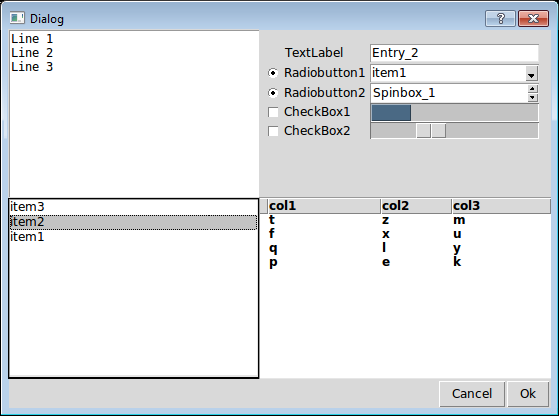
\includegraphics[width=0.49\textwidth]{img/tkinter-test}}
			\subfigure[wxPython]{\label{fig:wxpython}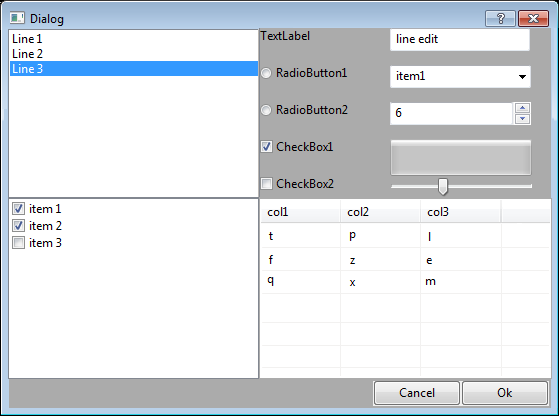
\includegraphics[width=0.49\textwidth]{img/wxPython-test}}
			\subfigure[PyQt]{\label{fig:pyqt}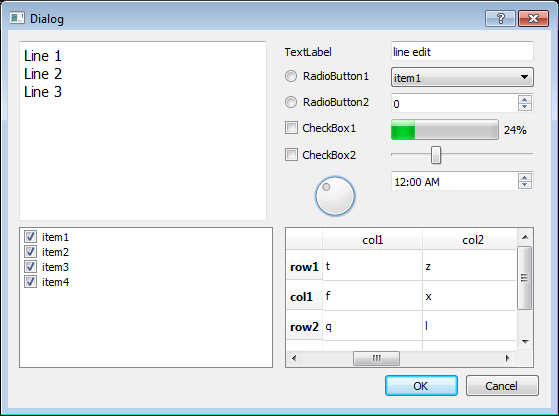
\includegraphics[width=0.49\textwidth]{img/pyqt-test}}
		\end{subfigmatrix}
		\caption{Сравнение библиотек графического интерфейса}
		\label{fig:gui-samples}
	\end{figure}
	
	Среди недостатков Tkinter часто выделяют сложность отладки. Также распространено мнение, что эта библиотека не в полной мере соответствует представлениям о современном интерфейсе. С другой стороны Tkinter входит в стандартную поставку Python, не требует установки дополнительных модулей, достаточно прост, гибок и функционален. 
	
	wxPython --- это библиотека, которую приходится устанавливать отдельно. Опытные разработчики отмечают относительно слабую проработку документации, сложность поиска справочной информации. В то же время wxPython страдает от некоторых проблем, связанных с переносимостью программы для работы под различными операционными системами. К положительным сторонам wxPython относят богатый состав типовых элементов и лучшее графическое оформление по сравнению с Tkinter. 
	
	Широкую известность получила кросплатформенная библиотека Qt, которая написана на C++ и изначально предназначена для этого языка. История этой библиотеки начинается с 1995 года, с тех пор библиотека регулярно обновляется, при этом устраняются ошибки, добавляются усовершенствования и нововведения. Документация библиотеки составлена тщательно, а большое число опытных пользователей охотно делятся рекомендациями и эффективными подходами использования средств библиотеки. Теперь воспользоваться преимуществами библиотеки можно и из языка Python. Программная библиотека PyQt представляет собой оболочку библиотеки Qt в Python классы. Удобство применения PyQt также обеспечивается наличием CASE (Computer-Aided Software Engineering) инструментов для этой библиотеки. Например, Qt Designer позволяет компоновать пользовательский интерфейс в том виде, в котором он будет представлен пользователю без необходимости писать программный код. Основной недостаток, который отмечают пользователи --- лицензионная политика разработчика библиотеки. Для свободного программного обеспечения используется лицензия GNU GPL, но для коммерческих проектов требуется приобретение платной лицензии \cite{PyQt}.
		
		
	\subsubsection{Библиотеки для работы с данными}	
	Для работы с данными применяется в целом типичный набор Python библиотек: Pandas, NumPy, SciPy, scikit-learn и Matplotlib. Первая библиотека используется для удобства преобразования и отображения табличных данных. NumPy в основном применяется непосредственно для реализации алгоритмов и матричных вычислений, например в NumPy входит функция SVD разложения. SciPy позволяет численно определять минимум заданной функции, что в частности используется для вычисления центра Минковского. Библиотека scikit-learn имеет в своём составе функцию для эффективного вычисления индекса ARI. Отображение данных в виде различного рода диаграмм (SVD, гистограммы, поля рассеивания) удобно реализовать при помощи библиотеки Matplotlib.
	
	\subsubsection{Тестирование}
	Тестирование --- важный этап разработки ПО. Правильно организованное тестирование способствует обеспечению высокого качества программного продукта а также сокращению времени на отладку. Наибольший эффект достигается при автоматизированном тестировании, что позволяет проверять работоспособность программы после каждого изменения в коде, тем самым все возникающие ошибки сразу же обнаруживаются. Следует понимать, что написание тестов также требует определённых усилий и для сложных программ невозможно обеспечить полное покрытие тестами всего кода. 
	
	В первую очередь необходимо составлять тесты на наиболее ответственные программные компоненты, от которых зависит работоспособность системы в целом. Таким компонентом в системе INDACT является модуль кластеризации. Ошибки в графическом интерфейсе, как правило, не столь значимы и критичны, они проявляются в ограниченном виде и слабо влияют на работоспособность незатронутых функций. К тому же их относительно легко обнаружить вручную. Тестирование графического интерфейса практически реализуемо, но в данном случае не целесообразно и излишне трудоёмко.
	
	Для тестирования модуля кластеризации применяется библиотека pytest. Преимущества этой библиотеки заключаются в богатом функционале, включающем в себя удобные функции для проверки утверждений, параметризацию тестов, подключаемые плагины, а также в генерации подробных отчётов и независимости от API (pytest не требует импорта модулей фреймворка). 
	
	Тесты основаны на сопоставлении результата работы разрабатываемого алгоритма и достоверной процедуры на заранее определённых данных. Под достоверной процедурой понимается способ кластеризации с высокой степенью доверия. Например, при фиксированных данных небольшой размерности можно провести вычисления вручную и сохранить результат в текстовый файл, который будет сверяться с результатом работы написанной программы. Второй вид достоверной процедуры --- использование сторонних Python библиотек для проверки частных случаев более общих алгоритмов. По такому пути можно пойти, например, при тестировании взвешенной версии \kmeans при $ p=\beta=2 $. Для этого надо сначала произвести аномальную кластеризацию и определить центры и число кластеров. Полученные кластеры используются как для инициализации разработанного алгоритма при $ p=\beta=2 $, так и для библиотечного \texttt{sklearn.cluster.KMeans}. Таким образом, в частном случае \imwkmeanspb является алгоритмом \kmeans и по этому частному случаю можно производить первичный контроль. Третий случай достоверной процедуры представляет собой использование MATLAB кода от авторов алгоритмов. Этот код запускается через командную строку в среде MATLAB  прямо во время выполнения теста. Результат возвращается путём захвата стандартного вывода. Конечно, третий способ предпочтителен, он не требует фиксации данных. Но не следует пренебрегать и первыми двумя, ведь и в коде авторов алгоритмов могут содержаться ошибки. 
	
	Приведем простой пример кода, который на самом деле используется для проверки работоспособности \AWard. 
	
	\lstinputlisting[caption={Тестирование \AWard},firstline=0,lastline=500,language=Python]{code/test_a_ward.py}	
	
	Первая строка импортирует тестируемый алгоритм, а вторая --- функцию проверки равенства разбиений. Эта функция способна определить фактическое равенство двух разбиений, даже если кластеры пронумерованы разными способами. Тестирующая функция \texttt{test\_a\_ward} принимает обобщённый параметр \texttt{data\_cs\_k\_star\_res}, значение которого определяется конфигурационным файлом и автоматически вставляется фреймворком pytest. Предаваемый параметр содержит ссылку на обрабатываемые данные и кластерную структуру, полученную при аномальной инициализации, а также терминальное число кластеров и результат выполнения достоверной процедуры. После распаковки обобщённого параметра происходит запуск алгоритма \AWard и сопоставление полученного результата с истинным разбиением при помощи функции \texttt{transformation\_exists}. Если существует такой способ перенумеровать полученное разбиение, чтобы в точности получить истинное, тест считается пройденным, в противном случае фреймворком pytest автоматически формируется отчёт об ошибке при тестировании с указанием различий в рассматриваемых разбиениях.
	
	\subsubsection{Средства дистрибуции}
	Распространение программ, написанных на Python, отличаются некоторой спецификой. Для того  чтобы программа заработала на компьютере заказчика требуется обеспечить все закономерности и установить необходимые библиотеки. Нельзя оставлять без внимание даже версии устанавливаемых библиотек, в некоторых случаях от этого зависит работает программа или нет. Всё вышесказанное относится и к самому интерпретатору Python. Такая ситуация, как правило, вызывает раздражение заказчика и отнимает ресурсы разработчиков на поддержку процесса установки. Существуют инструменты, которые фиксируют все зависимости разработанной программы и устанавливают их на компьютере пользователя в автоматическом режиме. Указанные инструменты не гарантируют безошибочного процесса установки, ведь сами библиотеки могут требовать наличие каких-либо дополнительных компонент, причём не обязательно Python. 
	
	Практически исключить возникновение указанных ошибок позволила следующая процедура формирования распространяемого пакета. Программист устанавливает у себя на рабочей машине две виртуальные операционные системы, той же версии, что и у заказчика. Установки какого либо программного обеспечения на одну из операционных систем не производится, назовём эту ОС контрольной. Вторая операционная система служит для создания распространяемого каталога бинарных файлов. В неё устанавливаются все библиотеки, необходимые для запуска INDACT. Утилита pyinstaller \cite{Pyinstaller} также отслеживает все зависимости программы, но при этом создаётся единый исполняемый файл, который включает в себя все выявленные библиотеки в той версии, которая установлена на данный момент. Полученный файл сохраняется в контрольной, ``чистой'' операционной системе. Если программа в контрольной ОС функционирует исправно, сформированный каталог бинарных файлов может быть отправлен заказчику без опасений относительно требуемого стороннего программного обеспечения. Заказчику останется только запустить полученный бинарный файл и начать работу.
	
	\subsection{Cтруктура системы}
	Вся программа INDACT разделена на два модуля. Первый модуль содержит функции, непосредственно реализующие различные алгоритмы кластеризации и не зависит от второго модуля, в котором находится код для отображения графического интерфейса. Такое решение позволяет разработать несколько реализаций интерфейса для написанной библиотеки кластеризации, причём необязательно графических и пользовательских. Например, можно разработать код, который будет являться MATLAB оболочкой и вызывать скажем, \dePDDP из этого математического пакета. 
	
	На рисунке \ref{fig:packages} показана структура модулей программы INDACT. На этой диаграмме отображаются только состав модулей и иерархия вложенности Python-пакетов, с помощью которых организованы исполняемые \texttt{.py} сценарии, при этом сами сценарии не отображаются. Два основных модуля --- \texttt{ect} и \texttt{ectgui} призваны разделить реализацию алгоритмов кластеризации и графического интерфейса, как это было упомянуто выше. 
	
	Модуль \texttt{ect} разделён на три пакета, имплементирующие различные функциональные аспекты. Отдельные пакеты группируют код для тестирования и код генератора данных, соответственно \texttt{tests} и \texttt{generators}. Пакет тестирования в свою очередь разбит на компоненты, относящиеся к тестированию конкретных алгоритмов, некоторые из которых для краткости на рисунке \ref{fig:packages} скрыты. Наиболее важный пакет модуля \texttt{ect} --- \texttt{clustering}, в котором сгруппированы сценарии для выполнения кластеризации. В отдельные пакеты выделены алгоритмы дивизивной и агломеративной кластеризации, при этом в пакете агломеративной кластеризации обособлены две группы сценариев, выполняющих этап аномального анализа: \texttt{ik\_means} и \texttt{p\_init} .
	
	\begin{figure}[h!]
		\centering
		\includestandalone[width=\linewidth]{tikz/packages}
		\caption{Структура пакетов программы INDACT}
		\label{fig:packages}
	\end{figure}
	
	Модуль \texttt{ectgui} имеет более простую, практически плоскую структуру, в которой каждый внутренний пакет соответствует коду, предназначенному для обработки определённого окна или графического элемента приложения. В программе INDACT применяются таблицы из библиотеки PyQt, основанные на моделях. Модель таблицы представляет собой \mbox{Python-класс}, который наследуется от \texttt{QtCore.QAbstractTableModel} и содержит определённые методы, управляющий поведением и наполнением таблицы. Эти классы и расположены в пакете \texttt{ectgui.tables.models}
	
	
	\begin{figure}[h!]
		\centering
		\begin{forest}
			pic dir tree,
			where level=0{}{% folder icons by default; override using file for file icons
				directory,
			},
			[ect	
			[clustering 
			[agglomerative 
			[ik\_means 
			[ik\_means.py, file]
			]
			[pattern\_initialization
			[ap\_init.py, file] 
			[ap\_init\_pb.py, file]
			] 
			[utils 
			[a\_ward\_cluster\_structure.py, file] 
			[a\_ward\_pb\_cluster\_structure.py, file] [agglomerative\_cluster\_structure.py, file] [imwk\_means\_cluster\_structure.py, file] 
			[nearest\_neighbor.py, file]] 
			[a\_ward.py,file] 
			[a\_ward\_pb.py,file]
			] 
			[divisive
			[utils
			[bikm\_r\_cluster\_structure.py, file]
			[depddp\_cluster\_strucutre.py, file]
			[direction.py]
			]
			[bikm\_r.py, file]
			[depddp.py, file]
			]
			[cluster\_structure.py,file]
			[common.py,file]
			]
			[generators [kovaleva.py, file]]
			[tests [...]]
			]
		\end{forest}
		\caption{Подробная структура модуля \texttt{ect}}
		\label{fig:ect-tree}
	\end{figure}	
	
	
	Рассмотрим структуру модуля \texttt{ect} в подробностях. На рисунке \ref{fig:ect-tree} показан состав \texttt{ect} с указанием файлов Python сценариев. Сценарии, осуществляющие тестирование, не представляют большого интереса в данной работе, поэтому они пропущены. В настоящий момент в составе библиотеки кластеризации имеется один реализованный генератор данных, который был описан в разделе \ref{subsec:generator}. Файл с кодом генератора находится в директории \texttt{generators}.
	
	На начальных этапах программа INDACT разрабатывалась в функциональном стиле, для каждого алгоритма была написана отдельная функция, которая принимала входные данные и необходимые аргументы, регулирующие работу алгоритма и возвращала результат в виде массива номеров кластеров, соответствующих исходным объекта. Однако, такой подход был признан неэффективным: некоторые реализуемые алгоритмы частично повторяют друг друга, что приводило или к копированию фрагментов кода, что естественно недопустимо, или к чрезмерной зависимости одних фрагментов кода от других. В первом случае при изменении какой-либо процедуры в одном алгоритме, например, при исправлении ошибки, все изменения приходится повторять и в скопированных фрагментах, что в свою очередь ведёт к возникновению новых проблем. Избыточная взаимозависимость кода замедляет процесс разработки и усложняет отладку. 
	
	С учётом вышеизложенных проблем было принято решение использовать преимущества объектного подхода. Были выделены классы для каждого из алгоритмов а также для обобщённой кластерной структуры. Под обобщённой кластерной структурой понимается совокупность групп объектов, заданная на известном множестве  объектов, для которой определены некоторые процедуры, в ООП называемые также методами, и характеристики (атрибуты). Примерами процедур являются добавление и удаление новой группы объектов, а среди характеристик можно выделить, например, общее число групп. Наследование от класса обобщённой кластерной структуры позволяет использовать исходные методы и добавлять новые. Например, для реализации дивизивных алгоритмов к обобщенной кластерной структуре добавляется метод выбора наилучшего кластера. Примечательно, что благодаря принципу полиморфизма, реализация нового метода может отличаться в зависимости от алгоритма: одна реализация понадобится для \dePDDP, другая --- для \BiKMR. При этом код, вызывающий метод останется неизменным. Обобщенная кластерная структура описана в файле \texttt{clustering/cluster\_structure.py}
	
	Как упоминалось ранее, модуль кластеризации разбит по принципу работы. В пакете \texttt{agglomarative} содержится код, реализующий алгоритмы \AWard и \AWardpb вместе со сценариями для выполнения аномальной инициализации. Первый этап аномальной инициализации реализован двумя классами, которые описаны в файлах \texttt{ap\_init.py} и \texttt{ap\_init\_pb}. Класс \texttt{APInitPB} для взвешенной аномальной инициализации наследуется от \texttt{APInit}, переопределяя при этом два метода. Также объектный подход позволил избавиться от необходимости реализации двух алгоритмов \ikmeans: обобщенный алгоритм,  использующий преимущества полиморфизма определён в файле \texttt{clustering/agglomerative/ik\_means/ik\_means.py}. Пакт \texttt{agglomerative.utils} содержит описание кластерных структур, специфичных для каждого алгоритма. Все эти описания наследуют и при необходимости переопределяют поведение обобщённой кластерной структуры. 
	
	Аналогичным образом устроен и пакет дивизивной кластеризации. В нём также алгоритмы описаны в соответствующих файлах Python-сценариев, а определение кластерных структур вынесено в пакет \texttt{divisive.utils}. 
	
	Работа модуля графического интерфейса в работе подробно рассматриваться не будет. Этот модуль в основном использует функционал библиотеки PyQt и, в отличии от модуля \texttt{ect}, не определяет каких-либо сложных алгоритмов, которые могли бы использоваться в других проектах. 
	
	\subsection{Структура входных данных}
	Входными данными для рассматриваемых алгоритмов кластеризации является таблица объект-признак. В программной реализации эта таблица представлена в виде NumPy-массива, который хорошо подходит для хранения матрицы числовых значений и операций над ними. В то же время при анализе данных специалисты часто сталкиваются с необходимостью работать с номинальными признаками, которые принимают строковые значения. Эта проблема решается на уровне модуля графического интерфейса. Изначально предназначенная для работы с разнородными табличными данными Python библиотека Pandas имеет в своём составе функционал для загрузки данных из текстовых файлов, что делает её очень удобной для применения в модуле \texttt{ectgui}. В библиотеке Pandas для набора данных принято название DataFarme. Преобразование DataFarme в массив NumPy осуществляется за один вызов метода, что также очень удобно. Входные данные загружаются из текстового файла библиотекой Pandas, после нормализации признаков осуществляется их конвертация в массив NumPy и выполнение алгоритма кластеризации. Загрузка данных в библиотеке Pandas реализована достаточно гибко и позволяет настраивать различные параметры, но в программе INDACT реализована загрузка только из файлов, в которых каждая строка соответствует признаку, а значения в столбцах разделяются запятыми. Как правило, такие файлы имеют расширение \texttt{.csv}, но на самом деле расширение не накладывает строгих ограничений на содержание файла, поэтому данные могут загружаться и из файлов с другими расширениями, например, \texttt{.dat}. Дополнительные требования к названию признаков и номинальным значениям приведены в руководстве пользователя. Для наглядности ниже приведена типовая структуа файла входных данных, скопированная из руководства пользователя: 
		
	\begin{tcolorbox}[colframe=black!50!black,coltext=black!25!black,colback=white,title=\textbf{Пример файла входных данных}]
		\verb|          name,      price,   diag,    cpu,    ram,   stype,   vendor |\\
		\verb|Meizu U10 32GB,   11990.00,    5.0,   1.50,   3072,     IPS,    Meizu |\\
		\verb|ZTE Blade A510,    7011.00,    5.0,   1.00,   1024,     IPS,      ZTE |\\
		\verb|Huawei P9 Lite,   14190.00,    5.2,   2.00,   2048,     IPS,   Huawei |\\
		\verb|Meizu M5 32GB ,   12990.00,    5.2,   1.50,   3072,     IPS,    Meizu |\\
		\verb|ZTE Blade L370,    4990.00,    5.0,   1.30,   1024,     TFT,      ZTE |\\
		\verb|BQ Aquaris M5 ,   18072.00,    5.5,   1.50,   3072,     IPS,       BQ |\\
		\verb|      ...     ,     ...   ,   ... ,   ... ,   ... ,     ...,       ... |\\	
	\end{tcolorbox}
	
	\subsection{Реализация алгоритмов}
	В данном разделе будут освещены нюансы реализации алгоритмов, приведены вычислительные схемы и фрагменты кода, где это необходимо.


	\subsubsection{Инициализация аномальными кластерами }
	Рассмотрение агломеративных алгоритмов следует начинать с аномальной инициализации, которая включает в себя два этапа: поиск аномальных кластеров и запуск \kmeans по найденным центрам кластеров. Диаграмма классов, реализующих первый  этап приведена на рисунке \ref{fig:ap-init-classes}. При составлении этой диаграммы стандартная нотация, предполагающая обозначение модификаторов доступа префиксными символами \mbox{(+,-,\#)} не используется, так как язык Python не определяет область видимости с помощью модификаторов. Вместо модификаторов доступа принято руководствоваться соглашениями, по которым специальные методы выделяются двумя подчёркиваниями спереди и сзади, например \texttt{\_\_init\_\_}, а скрытые атрибуты отмечаются одинарным подчёркиванием спереди, например, \texttt{\_origin}.
	
	Класс обобщённой кластерной структуры назван \texttt{ClusterStructure}, он содержит основные методы, которые одинаково работают в большинстве реализаций. Для создания объекта \texttt{ClusterStructure} в качеств аргументов требуется передать массив данных, на которых определена структура кластеров.
	
	\begin{figure}[h!]
		\centering
		\includestandalone[width=\linewidth]{tikz/ap-init-classes}
		\caption{Диаграмма классов для инициализации аномальными кластерами.}
		\label{fig:ap-init-classes}
	\end{figure}
	
	Абстрактный класс \texttt{AgglomerativeClusterStructure} добавляет три абстрактных метода, которые используются при реализации агломеративных алгоритмов. Эти методы определяют способ вычисления расстояний между двумя объектами, объектом и кластером и двумя кластерами.	Классы кластерных структур \texttt{AWardClusterStructure} и \texttt{AWardPBClusterStructure} реализуют эти методы в соответствии с описанными математическими формулами для алгоритмов \AWard и \AWardpb. Также эти классы определяют метод слияния двух кластеров, которые не используются для аномальной инициализации, но играют важную роль в агломеративных алгоритмах.
	
	Непосредственно алгоритм выделения аномальных групп содержится в классе \texttt{APInit}. При этом процедура вычисления глобального центра данных вынесена в отдельный метод, что позволяет переопределить его в классе \texttt{APInitPB}, наследующем \texttt{APInit}. Вычисление глобального центра данных в алгоритме аномальной инициализации для \AWardpb является задачей минимизации метрики Минковского, в отличие от  \AWard, где достаточно просто вычислить среднее. Благодаря наследованию и введению абстрактной кластерной структуры, \texttt{APInitPB} практически не содержит кода, определяющего последовательность выполнения вычислений, а лишь адаптирует эту последовательность под более общий случай. Поэтому далее рассмотрение ограничим классом \texttt{APInit}.
	
	При создании объекта \texttt{APInit} сохраняется ссылка на переданные в конструктор данные и целочисленный порог, определяющий минимальную численность аномальной группы. На каждой итерации работы алгоритма происходит исключение части объектов из рассматриваемых данных. Для сохранения взаимосвязи объектов, рассматриваемых на очередной итерации с исходными объектами в конструкторе инициализируется массив целочисленных индексов, длина которого равна длине исходных данных. При исключении объектов происходит одновременно и исключение соответствующих им индексов, поэтому всегда можно восстановить разбиение, полученное на исходных данных. Также в процессе инициализации вычисляется глобальный центр данных, остающийся неизменным на протяжении всего времени работы алгоритма, и создаётся пустая кластерная структура.
		
	В Python функции можно рассматривать как объекты. Чтобы сделать вызываемый объект-функцию, программисту необходимо объявить метод \texttt{\_\_call\_\_()}. Как можно видеть из диаграммы классов на рисунке \ref{fig:ap-init-classes}, объект класса \texttt{APInit} может быть вызван как функция. Такой механизм вызова алгоритмов принят во всей разработанной библиотеке кластеризации. На рисунке \ref{fig:ap-init} приведена схема вычислений, реализованная методом \texttt{APInit.\_\_call\_\_()}. На этой схеме опущены некоторые детали, несущественные для понимания работы. В целом синтаксис близок к синтексису Python, но в некоторых случаях он изменён для наглядности и сокращения.
	\begin{figure}[h!]
		\centering
		\includestandalone[width=\linewidth]{tikz/ap-init}
		\caption{Схема работы метода \texttt{APInit.\_\_call\_\_()}}
		\label{fig:ap-init}
	\end{figure}
	
	Входными данными метода являются массив данных и целочисленный порог, определяющий минимальное число объектов в аномальной группе. Первый блок вычислений производит инициализацию, определяя предельное число итераций внутреннего цикла, и другие переменные, используемые в работе алгоритма. Следующий блок задаёт главный цикл вычислений, итерации которого выполняются пока данные не исчерпаны. Внутри главного цикла определяется относительный индекс начального центра аномального кластера как индекс в текущих данных наиболее удалённого объекта. Для того чтобы на следующем шаге создать аномальный кластер из одного объекта требуется определить индекс этого объекта на исходных данных. Эта операция выполняется следующей строкой: \texttt{tcentroid\_i = index[tcentroid\_ri]}. После создания кластера, также определяется массив из логических переменных, который задаёт этот кластер на текущих данных. Количество итераций внутреннего цикла ограничено сверху переменной \texttt{MAX\_LOOPS}. Этот цикл, начиная с найденного центра, формирует аномальный кластер путём попеременной минимизации квадратичного критерия. Если процедура сошлась до достижения предельного числа циклов, поток выполнения возвращается главному циклу. В главном цикле, после проверки сформированного кластера на соответствие критерию минимальной численности, он сохраняется в кластерную структуру, после чего из данных и индекса исключаются те объекты, которые входят в только что полученный аномальный кластер. После завершения работы метода, кластерная структура содержит искомое разбиение.

	Аномальная инициализация с учётом весовых коэффициентов выполняется тем же кодом, но различаются реализации вызываемых методов. Класс \texttt{APInitPB} переопределяет поведение методов для создания кластерной структуры и вычисления глобального центра данных. Подставляя соответствующую кластерную структуру мы получаем другое поведение при вычислении расстояний между объектами и кластерами.
	
	Перейдём к рассмотрению алгоритмов \ikmeans и \imwkmeanspb. Оба эти алгоритма реализованны одним классом \texttt{IKMeans}, что стало возможно благодаря применению абстрактной кластерной структуры. Диаграмма классов приведена на рисунке \ref{fig:imwkmeans-classes}. Различия в алгоритмах обеспечиваются подстановкой кластерных структур разных классов. Для реализации \ikmeans используется та же кластерная структура \texttt{AWardClusterStructure}, что и для вычленения аномальных групп. Особенности учёта весовых коэффициентов вынуждают создать отдельную кластерную структуру для \imwkmeanspb. 
	
	Код класса \texttt{IKMeans} достаточно прост и он полностью приведён в листинге \ref{code:ikmeans}. Конструктор принимает кластерную структуру как аргумент, при этом данные извлекаются из объекта кластерной структуры. Также класс имеет свойство, которое обеспечивает доступ для чтения кластерной структуры. Объекты класса \texttt{IKMeans} одновременно являются функциями, вызов которой приводит к выполнению алгоритма. Главный цикл ограничен по числу итераций значением 500. Если решение не сошлось, возвращается результат в том виде, в котором он был получен к моменту исчерпания предела в 500 итераций. Внутри главного цикла формируется словарь, который каждому кластеру ставит в соответствие объекты, которые необходимо в него включить. Создание такого словаря неизбежно потому что формирование кластеров должно происходить одновременно, так как от этого в общем случае зависят веса признаков. Внутренний цикл наполняет упомянутый словарь, перебирая данные по одному объекту. Для каждого объекта в строке \ref{line:nearest-cluster} выбирается наиболее близкий кластер. Близость кластера к объекту определяется процедурой, заданной классом кластерной структуры, что обеспечивает повторное использование кода для обоих алгоритмов \AWard и \AWardpb. Новые кластеры создаются также по правилам, определённым кластерной структурой (см. строку \ref{line:new-clusters} листинга \ref{code:ikmeans}). Если созданные кластеры не равны, тем что были на предыдущей итерации, кластерная структура обновляется новыми кластерами. В противном случае процесс завершается выдачей номеров кластеров, соответствующи объектам.
	
		
	\begin{figure}[h!]
		\centering
		\includestandalone[width=\linewidth]{tikz/imwkmeans-classes}
		\caption{Диаграмма классов для интеллектуальной инициализации}
		\label{fig:imwkmeans-classes}
	\end{figure}
	
	\lstinputlisting[caption={Код класса \texttt{IKMeans}},label={code:ikmeans},firstline=0,lastline=500,escapechar=|,language=Python]{code/ik_means.py}	

	  
	\subsubsection{\AWard}
	Для увеличения производительности \AWard был применён алгоритм цепи ближайших соседей (nearest-neighbor chain) \cite{nnc}. На каждой итерации алгоритма \Ward происходит поиск двух ближайших кластеров и их объединение. Нахождение пары ближайших кластеров требует в общем случае квадратичного времени. В то же время очередная итерация не сильно изменяет кластерную структуру и большая часть расстояний, вычисленных на начальных этапах, долгое время остаётся неизменным. Чтобы использовать эту информацию для ускорения \Ward можно заранее вычислить ориентированный граф ближайших соседей (ГБС) и обновлять его  при обновлении кластерной структуры. Как раз по такому принципу и работает алгоритм цепи ближайших соседей. Начиная с произвольного объекта происходит обход ГБС до тех пор, пока не будут найдены два кластера, которые взаимно являются ближайшими соседями, после чего просходит их объединение. Для нового кластера вычисляются ближайшие соседи и ГБС обновляется соответствующим образом. Недостаток алгоритма цепи ближайших соседей состоит в том, что обход происходит в порядке, не соответствующем порядку объединения кластеров алгоритмом \Ward. При этом результирующая кластерная структура, всегда совпадает с результатом работы \Ward. 

	\begin{figure} % \ContinuedFloat
		\centering
		\subfigure[Граф ближайших соседей (ГБС) на исходных данных] {\label{fig:ncc1}\includestandalone[width=0.4\textwidth]{tikz/nnc/nnc-1}}
		\subfigure[Путь до первого объединения] {\label{fig:ncc5}\includestandalone[width=0.4\textwidth]{tikz/nnc/nnc-5}}
		\subfigure[Первое объединение и обновление ГБС] {\label{fig:ncc6}\includestandalone[width=0.4\textwidth]{tikz/nnc/nnc-6}}		
		\subfigure[Второй объединение и обновление ГБС] {\label{fig:ncc7}\includestandalone[width=0.4\textwidth]{tikz/nnc/nnc-7}}
		\caption{Графическая трассировка алгоритма ближайших соседей}
		\label{fig:nnc}
	\end{figure}	

	На рисунке \ref{fig:nnc} приведена трассировка алгоритма цепи ближайших соседей. Алгоритм следует по графу ближайших соседей, хотя полностью его на строит. Для некоторых произвольных данных рисунок \ref{fig:ncc1} изображает ГБС синими стрелками. Это сделано исключительно в иллюстративных целях. Алгоритмом выбирается некоторая произвольная начальная точка, в трассировке она обозначена как 1. Для начальной точки вычисляется ближайший сосед (точка 2). Так как для точки 2 ближайший сосед не является точкой 1, происходит переход в точку 2. Перебор продолжается по пути в ГБС (обозначен красным цветом) до тех пор, пока не будут найдены две точки, являющиеся взаимными ближайшими соседями. Этот момент изображён на рисунке \ref{fig:ncc5}, а найденными точками являются точки 4 и 5. На рисукне \ref{fig:ncc6} показано слияние точек 4 и 5 в бирюзовый кластер. После слияния процесс продолжается с того места, где было обнаружены точки, образующие кластер. Рисунок \ref{fig:ncc7} изображает добавление к бирюзовому кластеру точки 3, при этом не происходит повторного вычисления и сравнения всех расстояний между объектами, а только между последними в цепи ближайших соседей.
			
	\lstinputlisting[caption={Фрагмент кода, реализующего алгоритм цепи ближайших соседей},label={code:nnc},firstline=0,lastline=500,escapechar=|,language=Python]{code/nnc.py}	
	
	Фрагмент кода, реализующего алгоритм цепи ближайших соседей приведён в листинге \ref{code:nnc}. Этот фрагмент является методом \texttt{NearestNeighborChain} и превращает соответствующие объекты в объекты-функции. В строке \ref{line:nnc-stack} создаётся пустой список, который играет роль стека и хранит пройденных путь. Процесс объединения повторяется в главном цикле до тех пор пока остаются кластеры. Если стек опустел, из текущей кластерной структуры выбирается следующий кластер (см. строку \ref{line:nnc-next}) и он добавляется в стек. На каждой итерации из стека извлекается конечный кластер, для которого определяется ближайший кластер-сосед. Если сосед не может быть найден, выполнение алгоритма прерывается (строка \ref{line:nnc-break}). В том случае, если найденный сосед уже имеется в пройденном пути, то он объединяется с конечным кластером, при этом объединяемые кластеры извлекаются из стека, иначе сосед добавляется в стек. Цикл замыкается. После завершения цикла осуществляется сортировка найденной последовательности объединений по расстоянию между кластерами (строка \ref{line:nnc-sort}).
	
	При заданном начальном числе кластеров $ n $, время работы алгоритма ближайших соседей составляет $ O(n^2) $ \cite{nnc}. Несмотря на то, что описанная реализация требует сортировки результата, которая занимает линейно-логарифмическое время, асимптотическое время работы не изменяется: $ O(n^2+n \log(n))=O(n^2) $. 
	
	\subsubsection{\AWardpb}
	Реализация алгоритма \AWardpb не использует преимущества метода цепи ближайших соседей, так как в \AWardpb после каждого объедения происходит перераспределение весовых коэффициентов в кластерах и соответственным образом изменяются расстояния, что не может быть учтено в классической формулировке упомянутого метода. Так как все особенности вычисления расстояний в алгоритмах инкапсулируются классом кластерной структуры, то реализация \AWardpb имеет достаточно общий вид и состоит из зацикленной последовательности поиска ближайших кластеров и их объединения, как показано на рисунке \ref{fig:award-pb-alg}.

	\begin{figure}[h!]
		\centering
		\includestandalone[scale=0.8]{tikz/award-pb}
		\caption{Схема работы метода \texttt{AWardPB.\_\_call()\_\_}}
		\label{fig:award-pb-alg}
	\end{figure}
		
	Переменная \texttt{cs} является ссылкой на кластерную структуру \texttt{AWardPBClusterStructure} (см. рисунок \ref{fig:ap-init-classes}), а целочисленная переменная \texttt{k\_star} определяет максимальное число кластеров, которое требуется найти. Условный блок, изображённый на рисунке  \ref{fig:award-pb-alg} задаёт главный цикл и проверяет, достигнуто ли заданное число кластеров. Если, нет то выполняются внутренние операторы. Внутри цикла первый блок обработки отвечает за поиск индексов двух ближайших кластеров относительно расстояния, определяемого кластерной структурой. Второй блок получает объекты кластеров по индексу и осуществляет их слияние опять же с помощью вызова метода кластерной структуры.
			


	\subsubsection{\dePDDP}
	\subsubsection{\BiKMR}
%	\subsection{Кластерные структуры *}
	
	\newpage
	\section{Демонстрационный пример}
	
	В данном разделе описывается полный цикл работы программы на демонстрационных данных. Рассмотрены вопросы формирования данных из xml файла, их загрузка в программу, кластеризация и интерпретация результатов. Большое внимание уделено вопросу определения числа кластеров.
	
	\subsection{Формирование данных}
	
	Для демонстрации был сформирован набор данных о смартфонах, продаваемых интернет-магазином Озон, на основе xml файлов, открыто предоставляемых на веб-сайте \cite{ozon-data}. В листинге \ref{code:ozon} приведён фрагмент файла, из которого видна структура описания товаров. Этот файл содержит параметры моделей смартфонов, продававшихся в магазине в IV квартале 2017 года. Значения характеристик указываются между определёнными xml тегами, например, запись \texttt{<price>11990</price>} означает, что цена данной модели составляет 11 990 руб. Аналогичным образом указаны и остальные параметры модели. В одном xml файле записана информация по нескольким сотням моделей, описание каждой модели сгруппировано внутри тега \texttt{<offer>}.
	
	\lstinputlisting[caption={Фрагмент xml файла с описанием товара},label={code:ozon},firstline=0,lastline=500,language=Xml, texcl=true]{code/ozon.xml.old}	
	
	Вычленение интересующей нас информации из этого файла не составляет труда. Единственный параметр, который сохранён в неудобном формате --- частота процессора. Однако, задача извлечения частоты процессора из строки также была успешно решена с применением регулярных выражений. В автоматическом режиме с помощью Python-скрипта xml файл был преобразован в плоскую таблицу объект-признак. При подготовке данных выяснилось, что файл содержит описание 581 модели, но всего 386 из них обладают уникальными характеристиками, остальные отличаются только цветом.
	
	\subsection{Описание данных}
	Данные, используемые в демонстрационном примере, являются таблицей размерности 386 $ \times $ 4.  Описание признаков приведено в таблице \ref{tab:features}. Связи между некоторыми признаками показаны на графиках на рисунке \ref{fig:features-dep}.
	
	\renewcommand{\arraystretch}{1.25}
	\begin{table}[h!]
		\caption{Признаки данных}		
		\label{tab:features}
		\begin{tabular}{|C{0.04\textwidth}| C{0.20\textwidth} | L{0.40\textwidth} | C{0.24\textwidth}| }
			\hline \# & Название & Описание  & Единица измерения\\ 
			\hline 1 & price & Цена данной модели смартфона в IV квартале 2017 года & руб. \\ 
			\hline 2 & diag & Размер диагонали экрана & дюйм \\
			\hline 3 & cpu & Частота центрального процессора (ЦП) & ГГц \\			
			\hline 4 & ram & Объем оперативной памяти & Мб \\						
			\hline
		\end{tabular}
	\end{table}
	
	\begin{figure}[h!]
		\centering
		\subfigure[Зависимость цены от диагонали экрана] {\label{fig:fd1} 		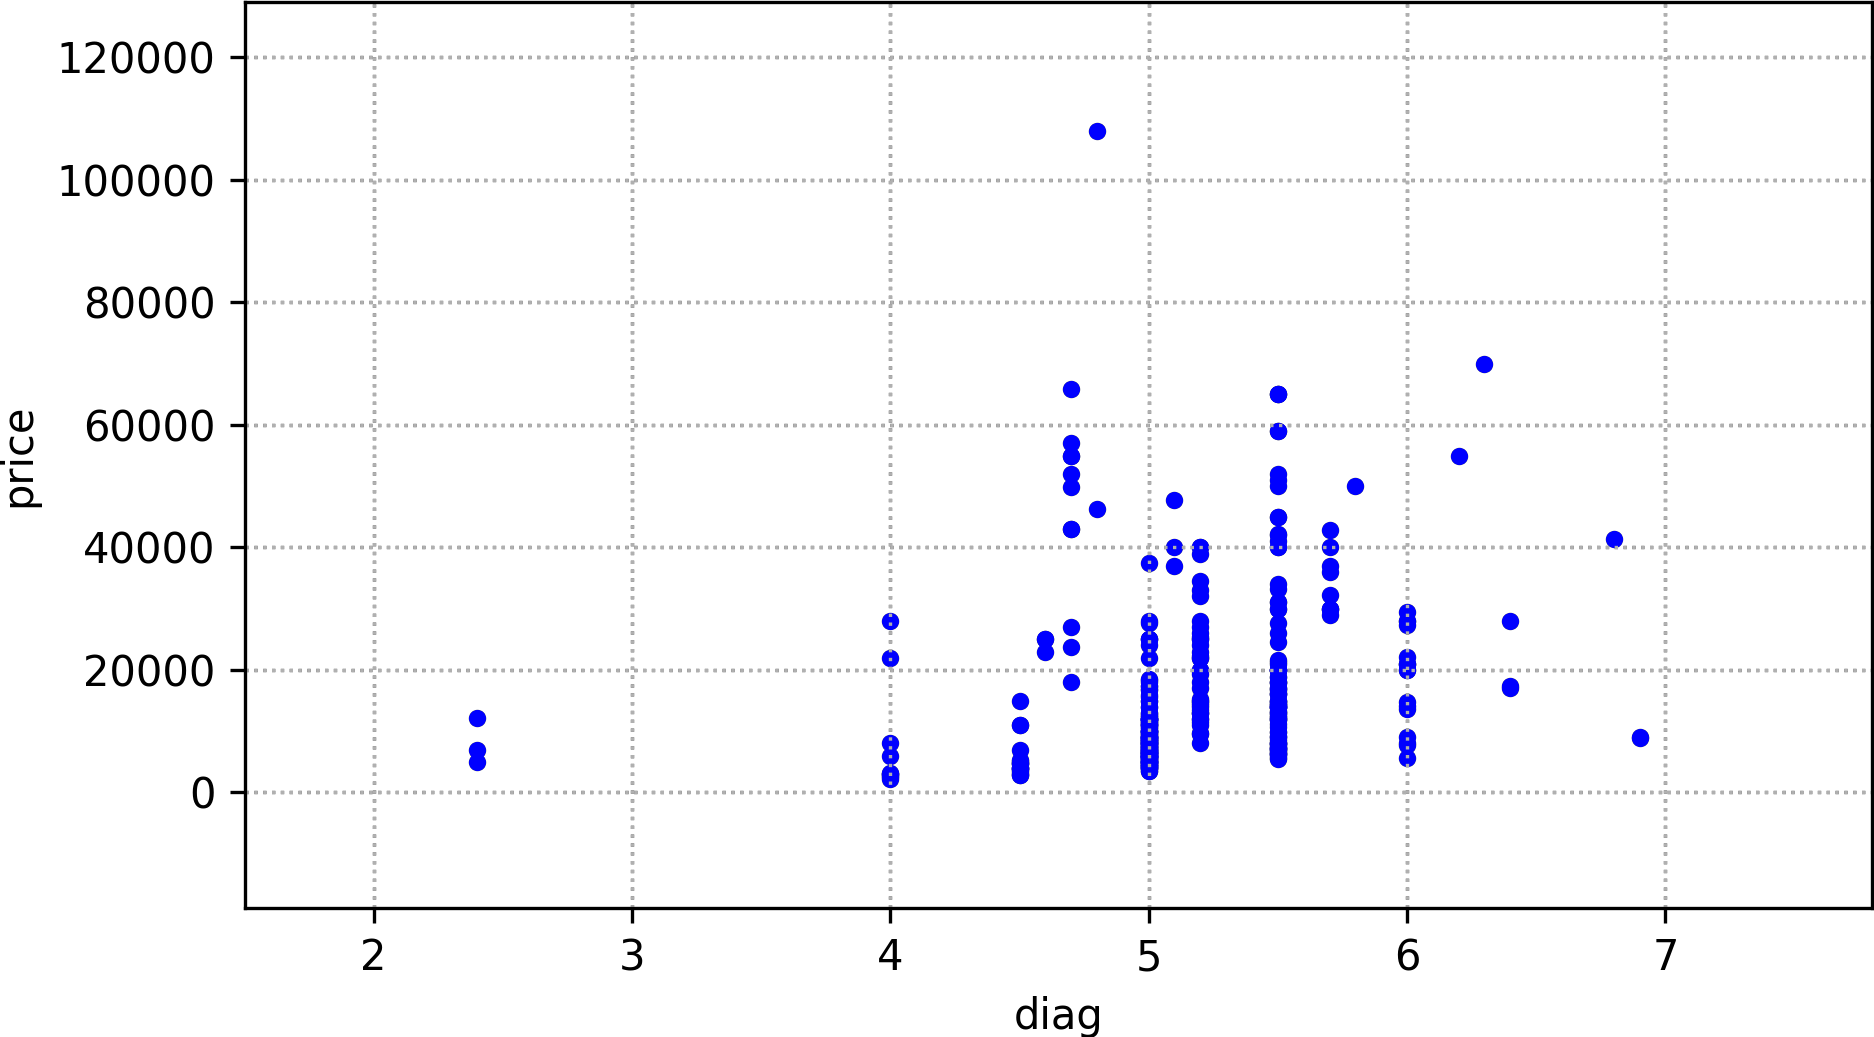
\includegraphics[width=0.48\textwidth]{img/dep/diag-price}}
		\subfigure[Зависимость объема ОЗУ от частоты ЦП] {\label{fig:fd2} 		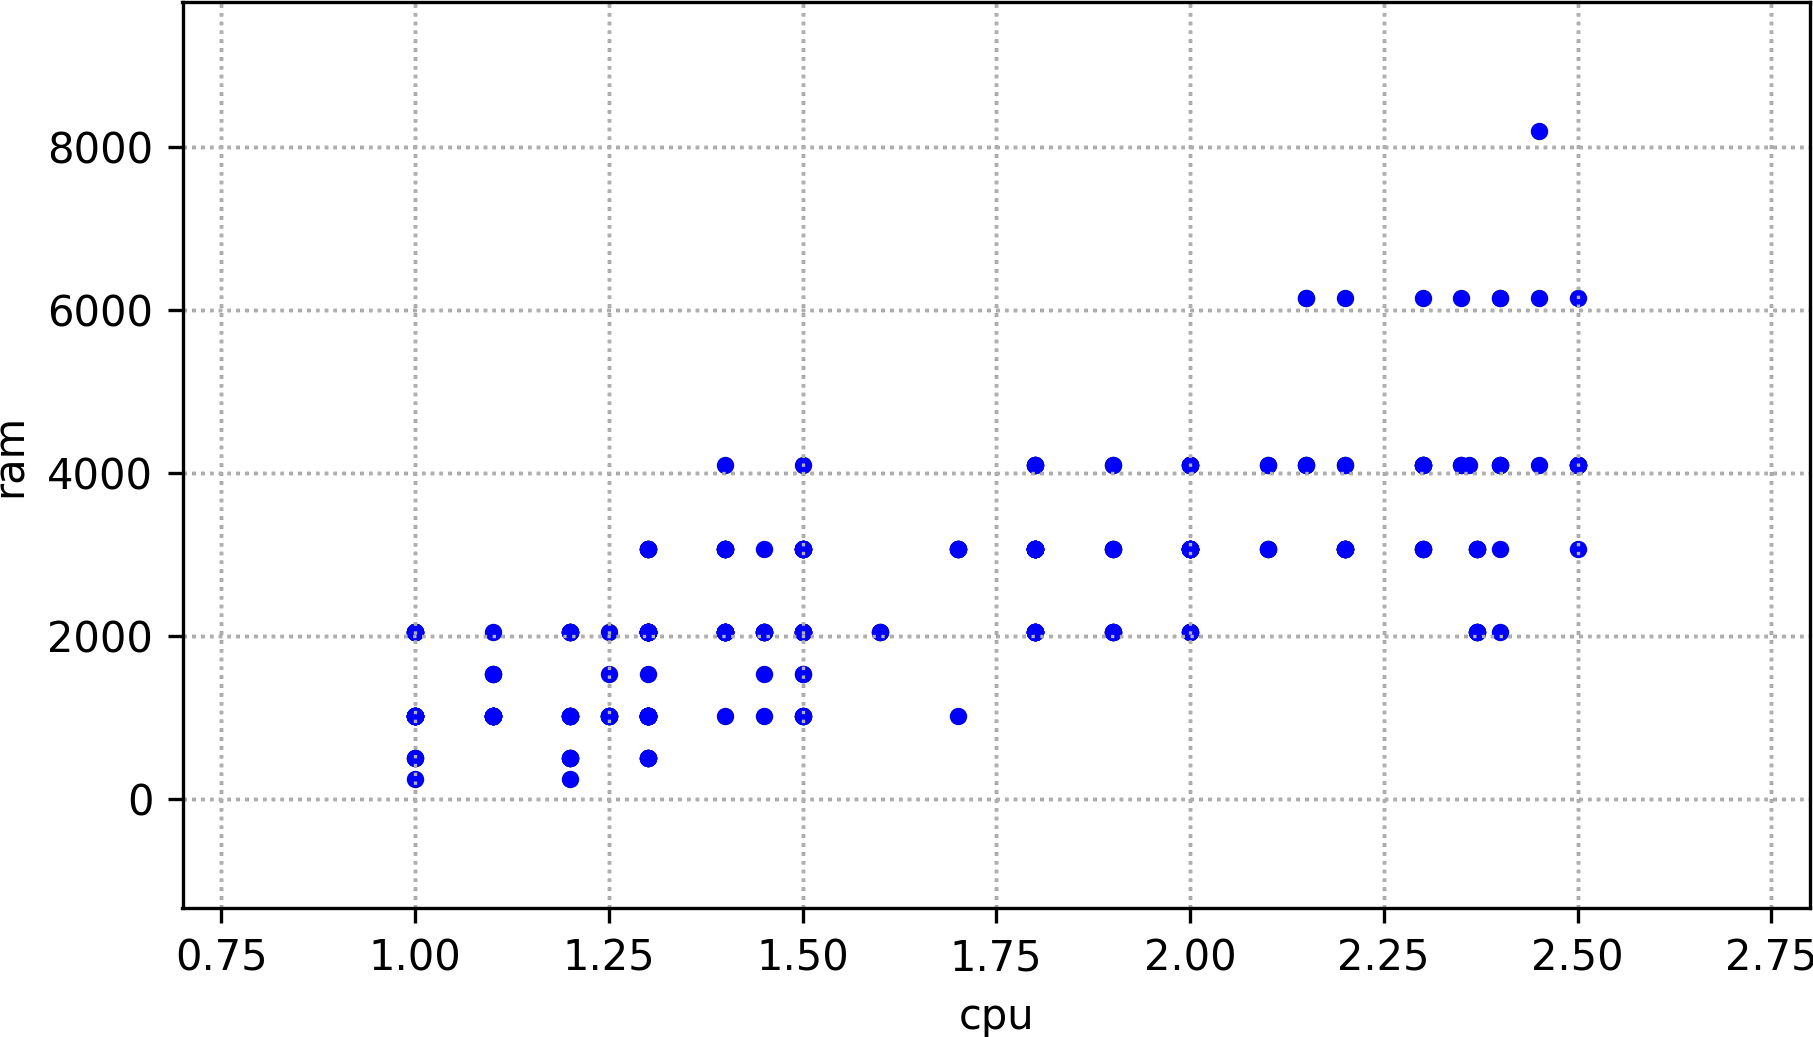
\includegraphics[width=0.48\textwidth]{img/dep/cpu-ram}}
		\subfigure[Зависимость цены от частоты ЦП] {\label{fig:fd3} 		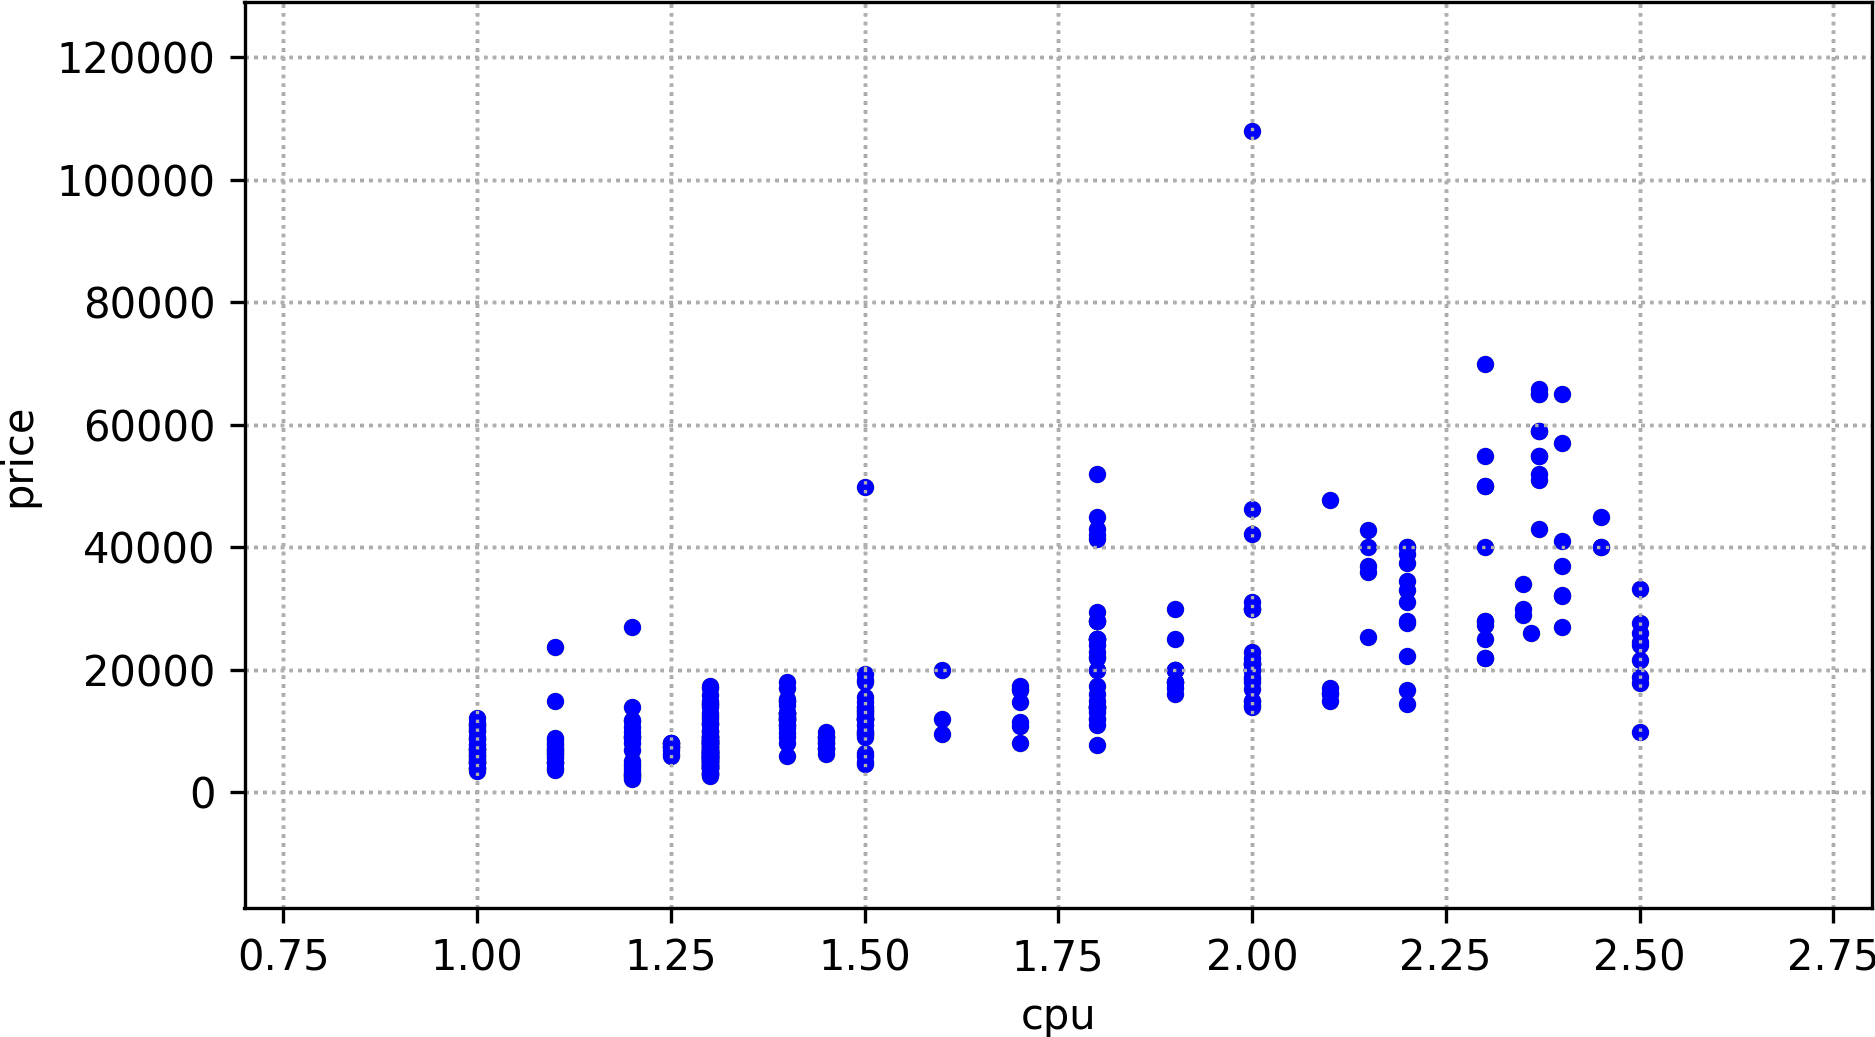
\includegraphics[width=0.48\textwidth]{img/dep/cpu-price}}
		\subfigure[Зависимость цены от объема ОЗУ] {\label{fig:fd4} 		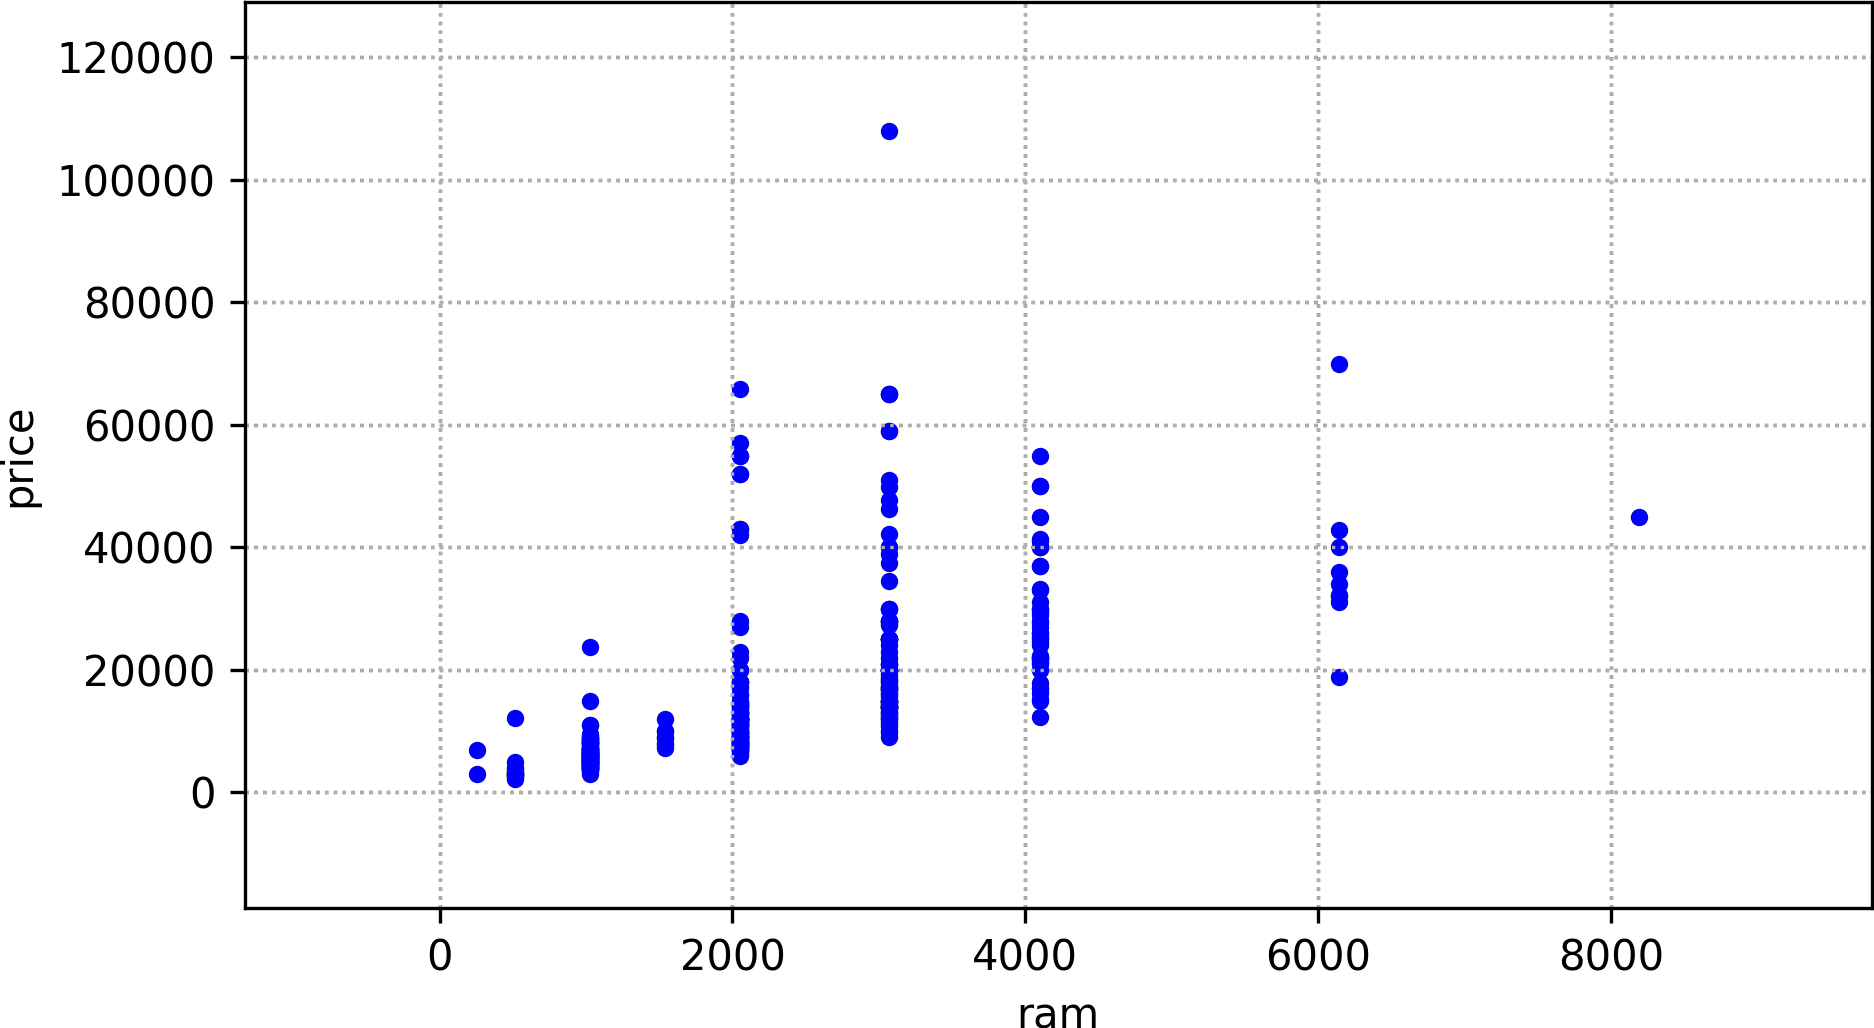
\includegraphics[width=0.48\textwidth]{img/dep/ram-price}}				
		\caption{Зависимости некоторых признаков}
		\label{fig:features-dep}
	\end{figure}	
	
	Ниже приведен фрагмент файла исходных данных, загружаемого в программу INDACT:
	\lstinputlisting[numbers=none,firstline=0,lastline=500,language={}]{code/smartphones.dat}
	
	\subsection{Нормализация}
	Значения признаков заданы в различных шкалах, поэтому требуется провести нормализацию данных. Как было описано раннее, функционал системы предполагает проведение нормализации с двумя параметрами: сдвиг и диапазон. Для рассматриваемых данных исходных предположений о способе нормализации нет, поэтому применена стандартная процедура с вычитанием среднего значения по столбцам и масштабированием по полуразмаху:
	\begin{gather*}
	Y_v'=\frac{Y_v-\frac{1}{N}\sum_{i=1}^{N}y_{iv}}{\frac{1}{2}(\max_{i} y_{iv}- \min_{i}y_{iv})},\;v=1,2,3,4
	\end{gather*}	
	\subsection{Кластеризация}
	Для кластеризации демонстрационных данных будут опробованы 4 алгоритма: \ikmeans, \dePDDP, \BiKMR, \AWard. Применение на выбранных данных алгоритма \AWardpb не обосновано, так как он в основном предназначен для случаев с сильно зашумлёнными данными.
	
	
	\renewcommand{\arraystretch}{1.5}

	\begin{table}[]
		\centering
		\caption{Попарный индекс ARI полученных разбиений}
		\label{tab:alg-ari}	
		\begin{tabular}{|c|c|c|c|c|c|}
			\hline
			 Число кластеров & Алгоритм & \ikmeans & \dePDDP & \BiKMR & \AWard \\ 
			\hline
			9 & \ikmeans  & 1 & 0.28 & 0.36  & 0.67  \\ 
			\hline
			4  & \dePDDP  & - & 1 & 0.25 & 0.46 \\ 
			\hline
			4   & \BiKMR  & - & - & 1 & 0.63 \\ 
			\hline
			4*   & \AWard & - & - & - & 1\\
			\hline
		\end{tabular} 
	\end{table}
	
       Главным является вопрос о числе кластеров. Для его решения мы применили три алгоритма, которые определяют число кластеров без участия пользователя. Алгоритмы dePDDP и BiKMR привели к числу кластеров, равному 4, тогда как алгоритм \ikmeans дал значительно большее число кластеров, 9. Алгоритм \ikmeans запускался при стандартном пороговом значении $ \Theta=1 $. Полученный результат согласуется с теоретической частью, в которой утверждалось, что \ikmeans при стандандартных настройках обнаруживает избыточное число кластеров. 
       Поэтому было принято, что число кластеров равно 4, после чего использовался алгоритм \AWard, выполняющий попарное объединение наиболее близких кластеров, полученных по методу \ikmeans, до тех пор, пока не получится 4 кластера. 

	Результаты попарного сравнения полученных разбиений с помощью индекса ARI сведены в таблице \ref{tab:alg-ari}. Число кластеров для алгоритма \AWard отмечено звёздочкой, это означает что оно фиксируется пользователем при запуске.  Как видно, разбиение по методу   \AWard наиболее похоже на остальные. Поэтому далее предлагается рассматривать именно это разбиение.
	
	\begin{figure}[h!] % \ContinuedFloat
		\centering
		\subfigure[\ikmeans] {\label{fig:svd-sample1}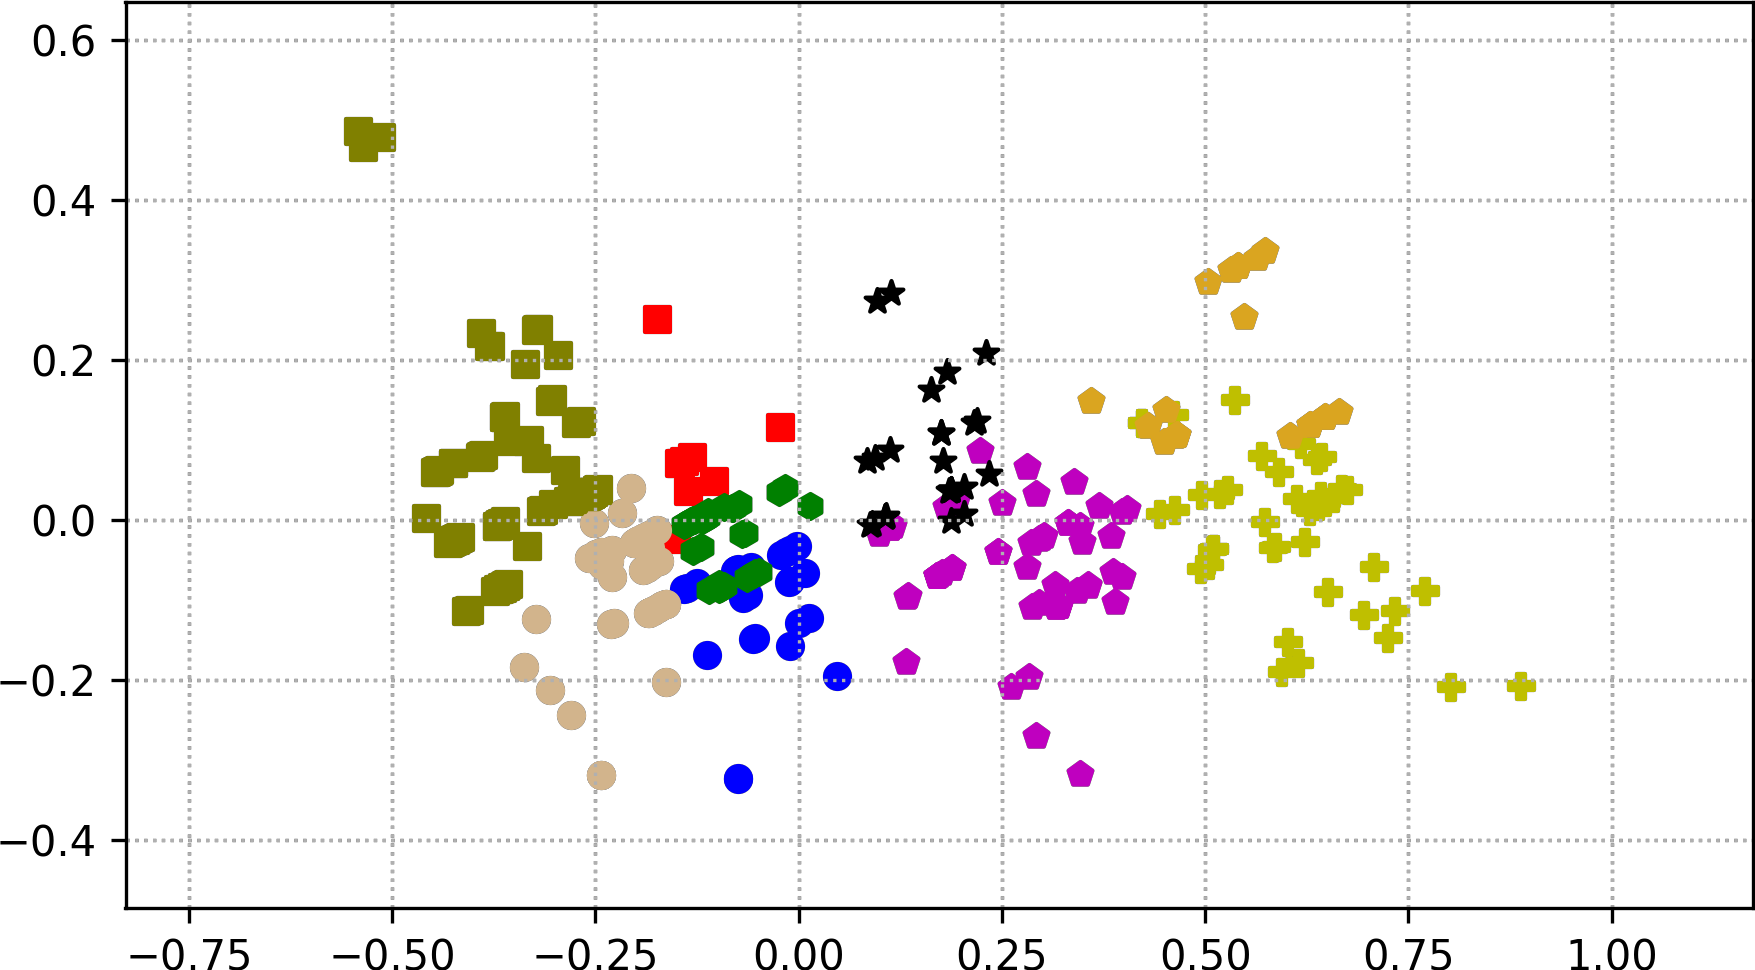
\includegraphics[width=0.48\textwidth]{img/svd/ikmeans-svd}}
		\subfigure[\dePDDP]  {\label{fig:svd-sample2}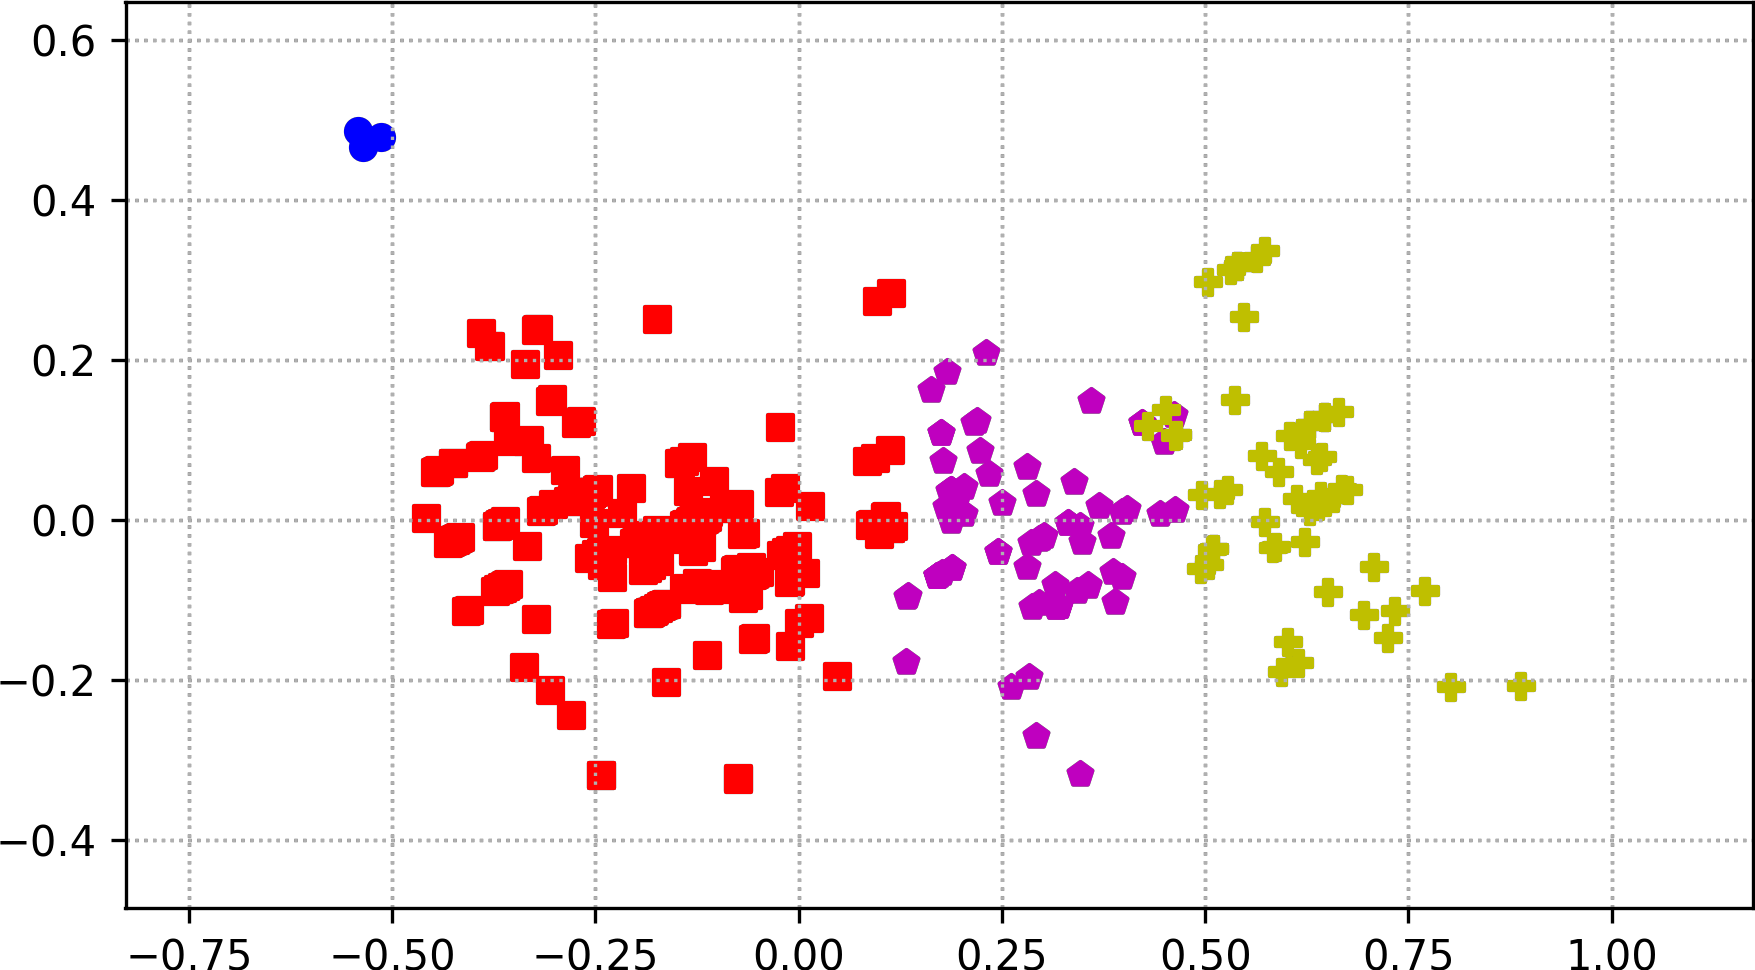
\includegraphics[width=0.48\textwidth]{img/svd/depddp-svd}}
		\subfigure[\BiKMR]   {\label{fig:svd-sample3}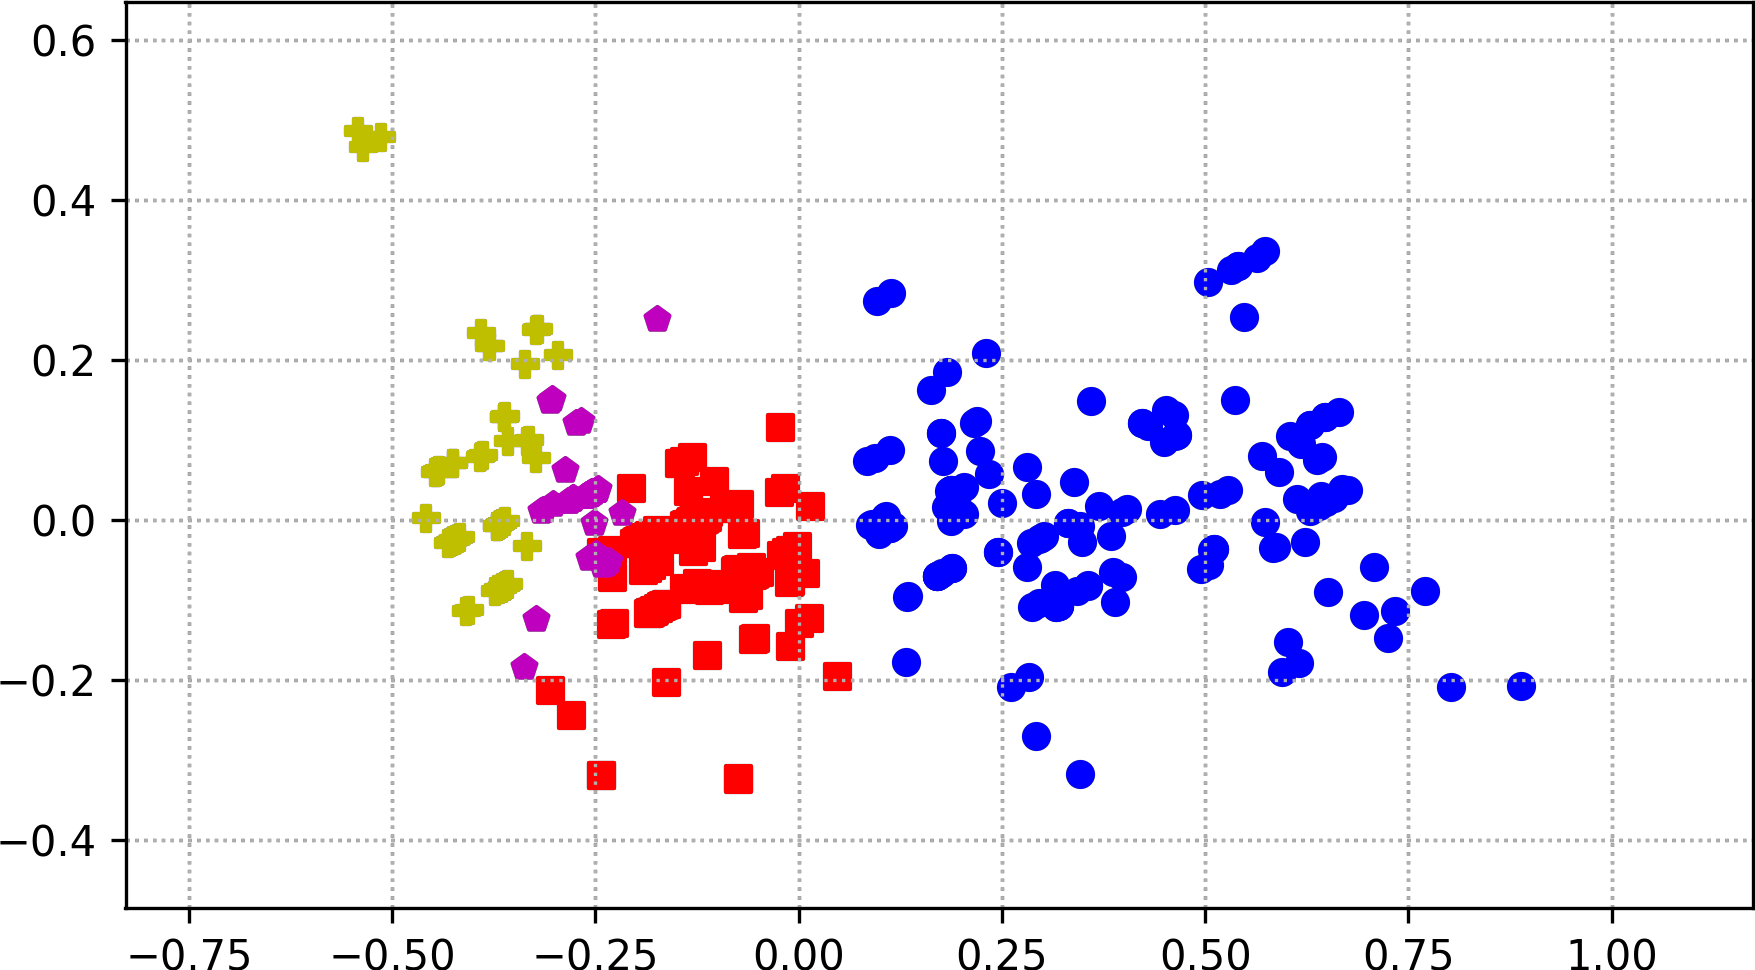
\includegraphics[width=0.48\textwidth]{img/svd/bikmr-svd}}		
		\subfigure[\AWard]   {\label{fig:svd-sample4}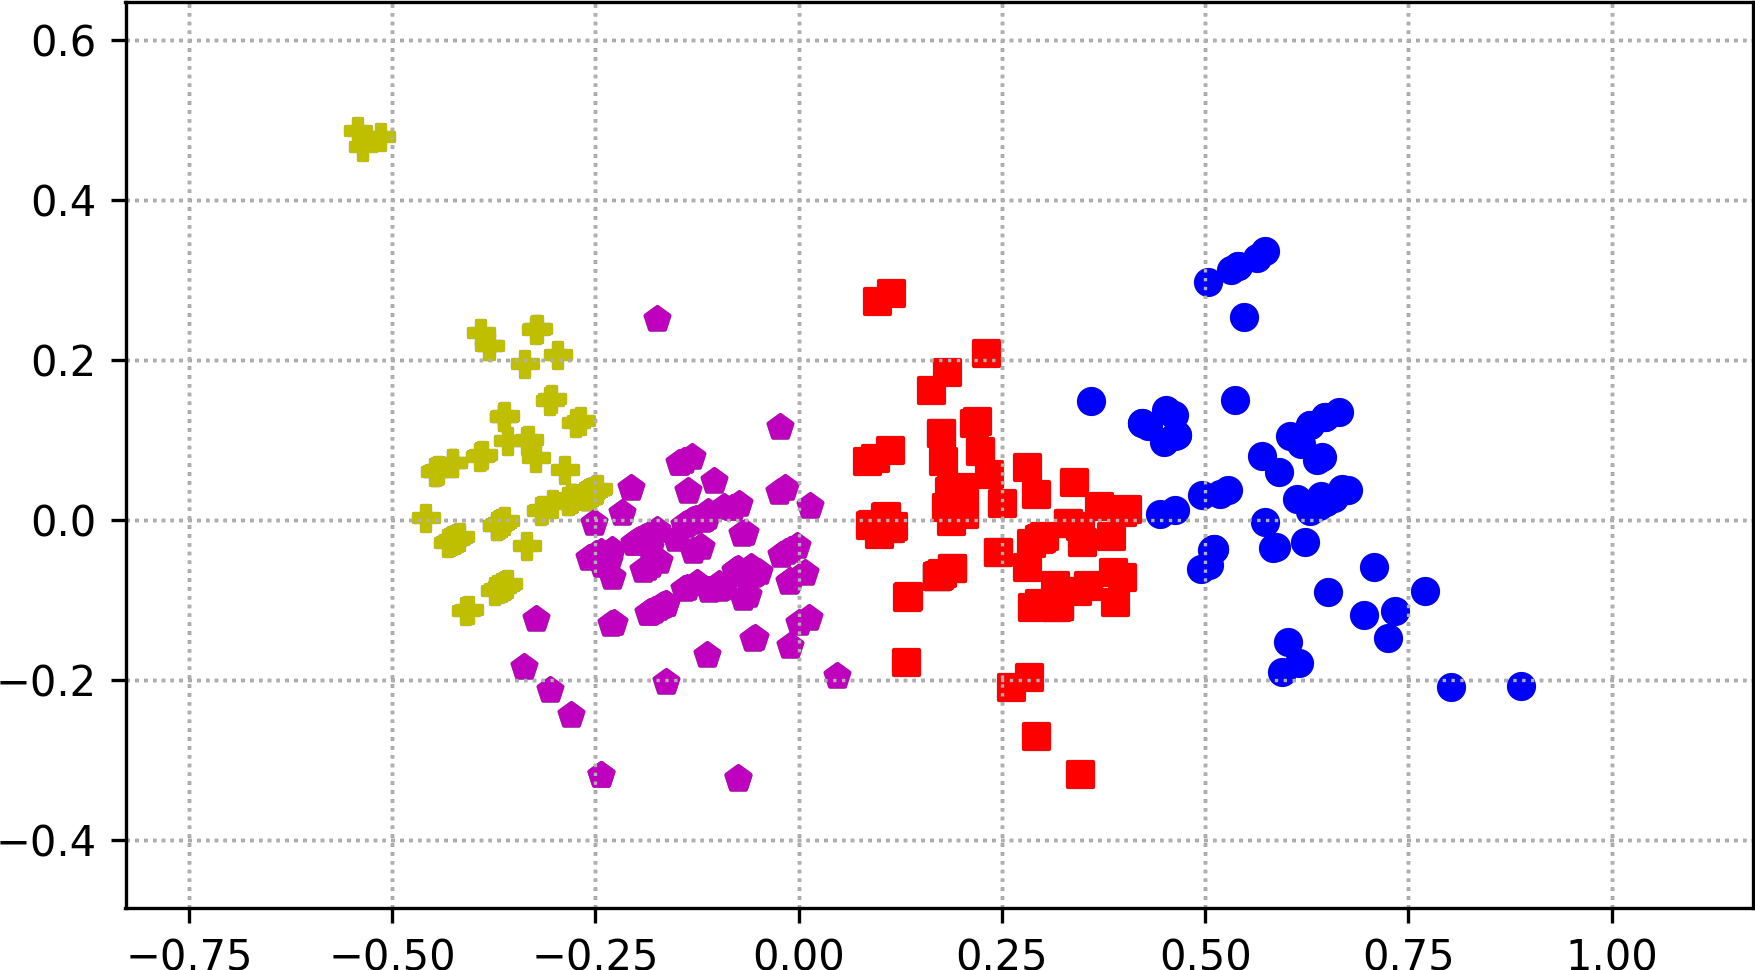
\includegraphics[width=0.48\textwidth]{img/svd/award-svd}}
		\caption{SVD диаграммы полученных разбиений}
		\label{fig:svd-sample}
	\end{figure}	
		
	\subsection{Интерпретация результатов}		
	Проанализируем  кластеры, полученные алгоритмом \AWard.
Для этого рассмотрим таблицу отдельных кластеров для нормализованных данных (далее эту таблицу).
Как видно, в кластере 1 (62 объекта) доминирует значение 0.496 признака "Частота ЦП" - это значит, что данный кластер, в основном, выделяется этим признаком - в него входят смартфоны с максимальной частотой ЦП (2.321 ГГерц, как видно из соответствующей таблицы средних значений в исходных признаках - ее тоже надо привести). Оказывается, остальные кластеры также характеризуются доминированием этого признака: 0.205 (кластер 2б 82 объекта), -0.139 (кластер 3, 132 объекта) и -0.266 (кластер 4, 110 объектов), причем остальные признаки ему подстать - слегка больше среднего в кластере 2, слегка меньше среднего в кластере 3 (правда, здесь Диагональ на уровне среднего) и меньше среднего, особенно по объему ОЗУ, в кластере 4. В целом, можно утверждать, что расслоение моделей произошло в основном по признаку Частота ЦП - для кластеров характерны значения 2.321, 1.885, 1.369 и 1. 179, соответственно. Рис.   иллюстрирует это заключение.

	\begin{figure}[h!] % \ContinuedFloat
		\centering
		\subfigure[\dePDDP]  {\label{fig:interp2}\includestandalone[width=0.98\textwidth]{tikz/interpretation-depddp2}}
		\subfigure[\BiKMR]   {\label{fig:interp3}\includestandalone[width=0.98\textwidth]{tikz/interpretation-bikmr}}
		\subfigure[\AWard]   {\label{fig:interp4}\includestandalone[width=0.98\textwidth]{tikz/interpretation-award}}
		\caption{Относительное отклонение от среднего признаков в кластерах}
		\label{fig:interp}
	\end{figure}	

Можно посмотреть на разбиение по методу \dePDDP как наиболее отличающееся от остальных согласно таблице (АРИ). По той же методике рассматриваем таблицу центров кластеров в нормализованных признаках (см. Таблицу...). Кластер 1 содержит всего 3 модели, которые выделяются уменьшенными значениями всх параметров, особенно Диагональ экрана, -0.614, т.е. 2.4 дюйма. Остальные три кластера более или менее соответствуют, по характеристикам их центров, кластерам 1, 2, 3 по методу \AWard, рассмотренным выше. ОБращает на себя внимание кластер 2 по методу \dePDDP, объединивший более половины выборки, 253 модели - отсюда и отличия от остальных разбиений.
	\section{Заключение}	
	Программная система интеллектуальной кластеризации INDACT включает в себя модуль графического интерфейса и библиотеку из 5 современных алгоритмов кластер-анализа, а также средств анализа полученных кластеров. С помощью графического интерфейса INDACT позволяет проводить отбор признаков, нормализацию данных, первичный анализ с помощью полей рассеивания и гистограмм, а также запускать выполнение реализованных алгоритмов кластеризации. На основе полученных результатов кластеризации пользователь может сгенерировать подробный отчёт для дальнейшего анализа и выводов. Библиотека алгоритмов содержит три дивизивных метода: \ikmeans, \dePDDP и \BiKMR и два агломеративных: \AWard и \AWardpb. Для каждого из алгоритмов описаны особенности и рекомендуемая область применения.
	
	Система INDACT написана с учётом современных тенденций в области разработки программного обеспечения и с применением передовых технических приёмов и инструментов. Код программы написан на высокоуровневом популярном языке программирования Python и опирается на принципы объектного подхода для увеличения степени повторного использования вычислительных процедур. Разработка пользовательского интерфейса произведена в графическом редакторе, что позволило ускорить процесс создания системы. 
	
	Разработанная система позволит облегчить применение реализованных алгоритмов для специалистов, не обладающих углублёнными знаниями в кластер-анализе.
	
	Усовершенствование системы возможно в разных направлениях, из которых следует отметить следующие три: развитие функционала и добавление новых возможностей; испытания программы в реальных условиях с целью выявить пользовательские предпочтения по проведению и использованию результатов  кластер-анализа; доработка автоматических тестов для увеличения покрытия и включения в покрытие графического интерфейса. 



	\newpage
	\appendix
	
	\setcounter{section}{0}	
	\titleformat{name=\section}[display]
	{\normalfont\centering\bfseries}
	{\MakeUppercase{Приложение} \thesection}
	{0pt}
	{}
	\addcontentsline{toc}{section}{Приложения}	
	
	\section{Интерпретация кластеров \ikmeans}\label{app:A}
	
	\begin{figure}[h!]
		\centering
		\subfigure  {\label{fig:interp-ik-2}\includestandalone[width=0.98\textwidth]{tikz/interpretation-ikmeans2}}
		\caption{Относительное отклонение от среднего признаков в кластерах}
		\label{fig:interp-ikmeans}
	\end{figure}

	\section{Относительный вклад кластеров в признак}\label{app:B}
	
	\begin{figure}[h!] % \ContinuedFloat
		\centering
		\subfigure[\dePDDP]  {\label{fig:interp-rfc-2}\includestandalone[width=0.48\textwidth]{tikz/interpretation-depddp2-rfc}}
		\subfigure[\BiKMR]   {\label{fig:interp-rfc-3}\includestandalone[width=0.48\textwidth]{tikz/interpretation-bikmr-rfc}}
		\subfigure[\AWard]   {\label{fig:interp-rfc-4}\includestandalone[width=0.48\textwidth]{tikz/interpretation-award-rfc}}
		\caption{Относительный вклад кластеров в признак}
		\label{fig:interp-rfc}
	\end{figure}
	
	\begin{figure}[h!] % \ContinuedFloat
		\centering
		\subfigure[\ikmeans]  {\label{fig:interp-rfc-1}\includestandalone[width=0.98\textwidth]{tikz/interpretation-ikmeans-rfc}}
		\caption{Относительный вклад кластеров в признак}
		\label{fig:interp-rfc-ikmeans}
	\end{figure}
	

	\titleformat{\section}{\normalfont\fontsize{16}{0}\bfseries}{\thesection}{1em}{}
	
	\bibliography{bibliography}
	
\end{document}
